\chapter{LFV HIGGS DECAY SEARCH RESULTS}

The results can be extracted after applying the selection criteria and with the full consideration of the relevant systematics.  In both $\Hmuhad$ and $\Hehad$ analysis, a maximum likelihood fit is performed to derive the expected and observed limits.  Each category in the analysis is fitted separately and then combined. Systematic uncertainties are used as nuisance parameter in the fittings.  The upper limits on signal branching faction with $\textrm{CL}_{\textrm{s}}$ criterion are set with asymptotic formula. 

\subsection{Results in $\Hmuhad$ search}

In the lepton flavour violation $\Hmuhad$ search at central of mass energy of 13 TeV, the analysis is performed in two parallel searching method, the $\mcol$ fit analysis and BDT fit analysis. After the selection in the $\mcol$ fit analysis and adjusting all of distribution by the fit,  the distribution of the signal and background discriminant variable $\mcol$ is shown in Figure.~\ref{fig:cutbasedpostfit}. In the BDT fit analysis, the BDT discriminator is used as the variable to distinguish signal from background.  After fitting to all of the distributions, the observed data versus the expected backgrounds is shown in Figure.~\ref{fig:bdtbasedpostfit}. No excess over the backgrounds is observed in both of the methods. The expected and observed median upper limits at 95\% CL and the best fit branching fraction in the $\Hmuhad$ search with the $\mcol$ fit analysis is shown in Table.~\ref{tab:expected_limits_CutBased_MuTau}  and the result of the BDT fit analysis is shown in Table.~\ref{tab:expected_limits_BDTMethod2_MuTau}. 

The search in $H \to \mu \tau$ with CMS 13 TeV, 36 $\textrm{fb}^{-1}$ data is motivated by the previous CMS search on the 8 TeV dataset with 19.7 $\textrm{fb}^{-1}$ $H \to \mu \tau$, in which a significance of 2.4 standard deviation excess of data with respect to the SM background-only hypothesis was observed. This thesis describes the $\Hmuhad$ search, which combined together with another search for $H \to \mu\tau_{e}$~\cite{paper:13TeVsearch}, where the tau lepton decays electronically to an electron, instead of tau hadronically decay, provides the most sensitive search for $H \to \mu \tau$. The combined result is shown with the BDT fit analysis and $\mcol$ fit analysis separately in Figure.~\ref{fig:cutbasedpostfit}. No evidence of excess is found in this combined result. Compared with the prevous 8 TeV result, the new upper limits on the signal branching fraction improved a factor of 5. The BDT fit analysis is more sensitive than the the $\mcol$ fit analysis. The new and tighter limit result comes from the BDT fit analysis.  

The constrains on flavour violating Yukawa couplings can be derived from the limits on branching fraction of  LFV Higgs decay. The exact relationship between Yukawa couplings and branching fraction of LFV Higgs decays is shown in section.~\ref{effective_field}. The 125 GeV Standard Model Higgs  decay width is taken as $\Gamma_{\mathrm{SM}}=4.1\textrm{MeV}$~\cite{Denner:2011mq}.In BDT fit analysis, the 95\% CL upper limit on the Yukawa coupling is $\sqrt{Y_{\mu\tau}|^2 + |Y_{\tau\mu}^2|}<1.43\times 10^{-3}$ and in $\mcol$ fit analysis, $\sqrt{Y_{\mu\tau}|^2 + |Y_{\tau\mu}|^2}<2.05\times 10^{-3}$. The upper limit on Yukawa couplings of BDT fit analysis is shown in Figure.~\ref{fig:Yukawas}. The comparison with the previous experimental search and theoretical naturalness results is also shown in the plot. 


\begin{figure}[htbp] 
     \centering
     \subfigure[0 jet]{ 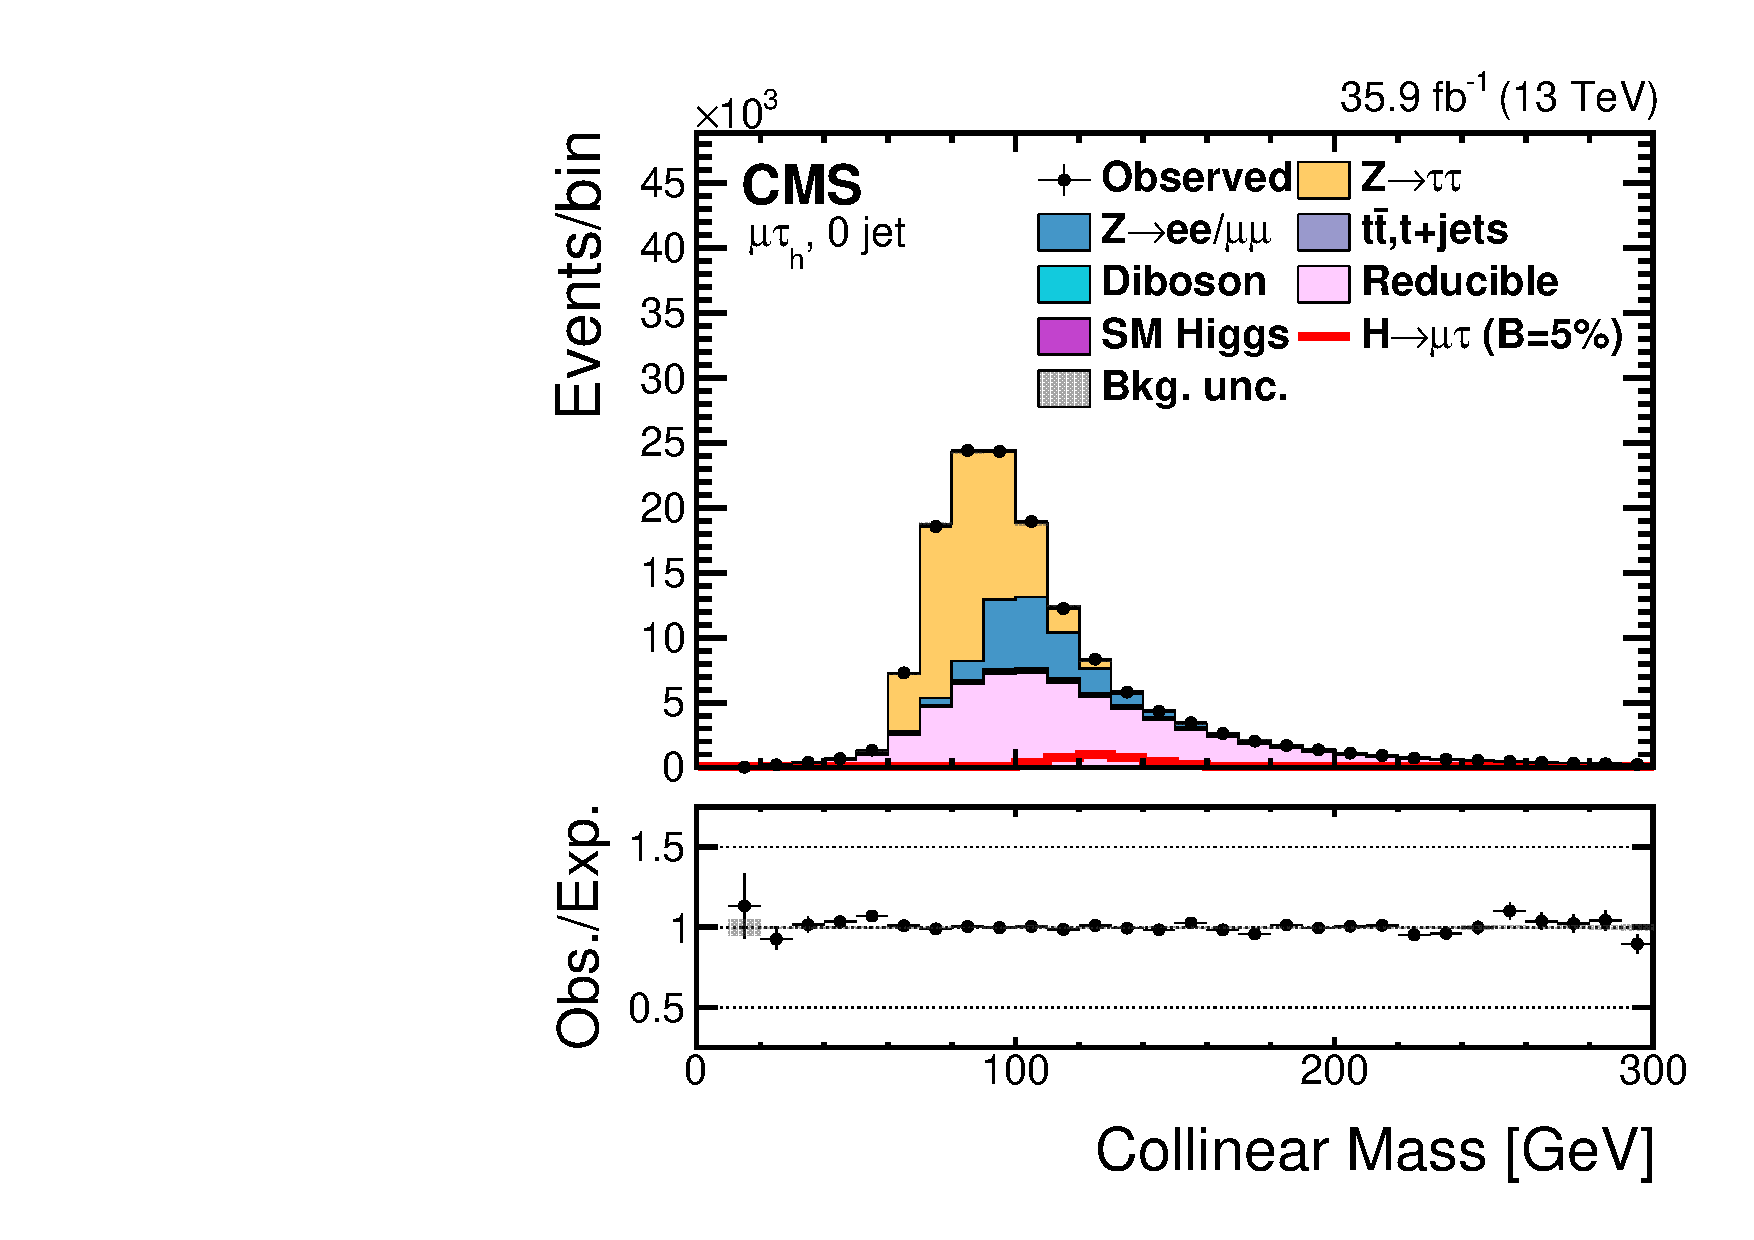
\includegraphics[width=0.4\textwidth]{chapter8/mutau_HMuTau_mutauhad_1_2016_postfit_COLMASS.pdf}}
     \subfigure[1 jet]{ 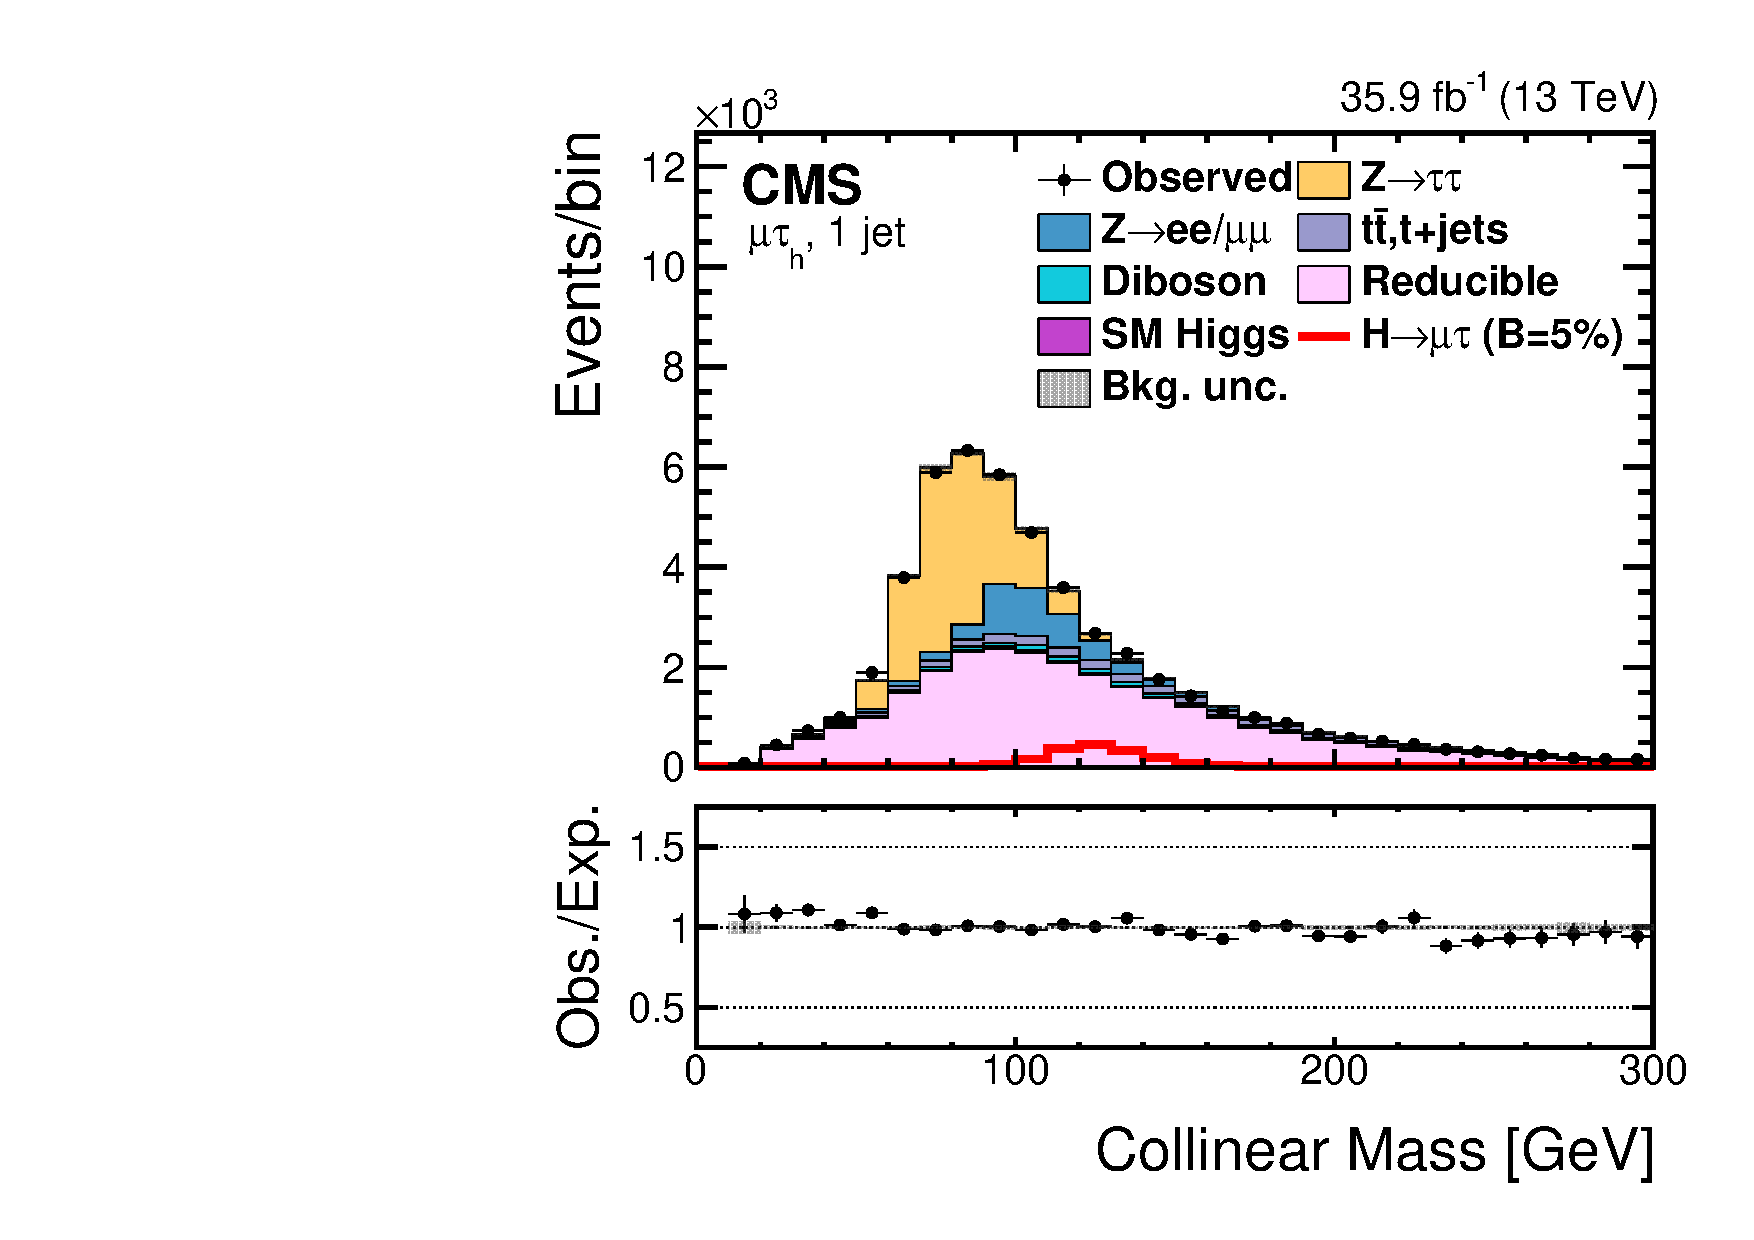
\includegraphics[width=0.4\textwidth]{chapter8/mutau_HMuTau_mutauhad_2_2016_postfit_COLMASS.pdf}}\\
     \subfigure[2 jets, gg-enriched]{ 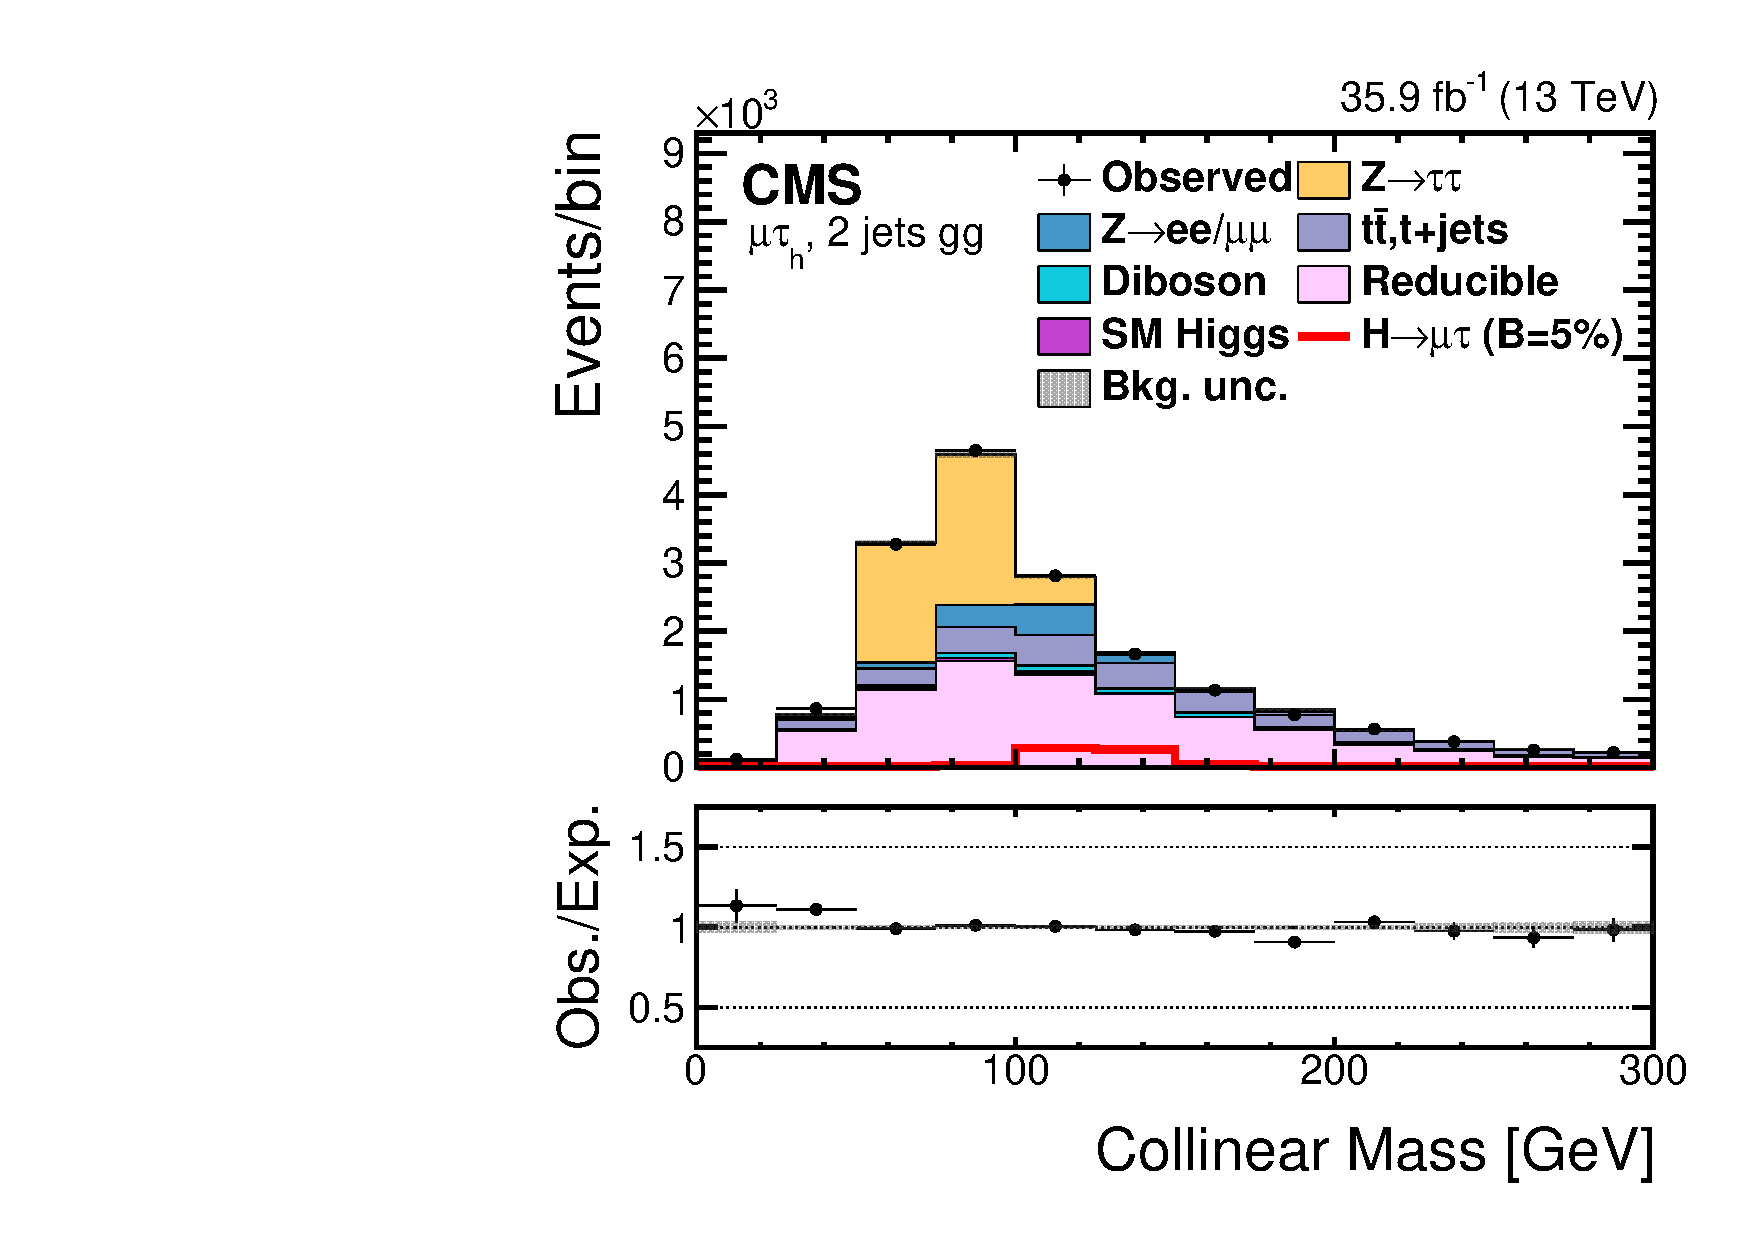
\includegraphics[width=0.4\textwidth]{chapter8/mutau_HMuTau_mutauhad_3_2016_postfit_COLMASS.pdf}}
     \subfigure[2 jets, VBF-enriched]{ 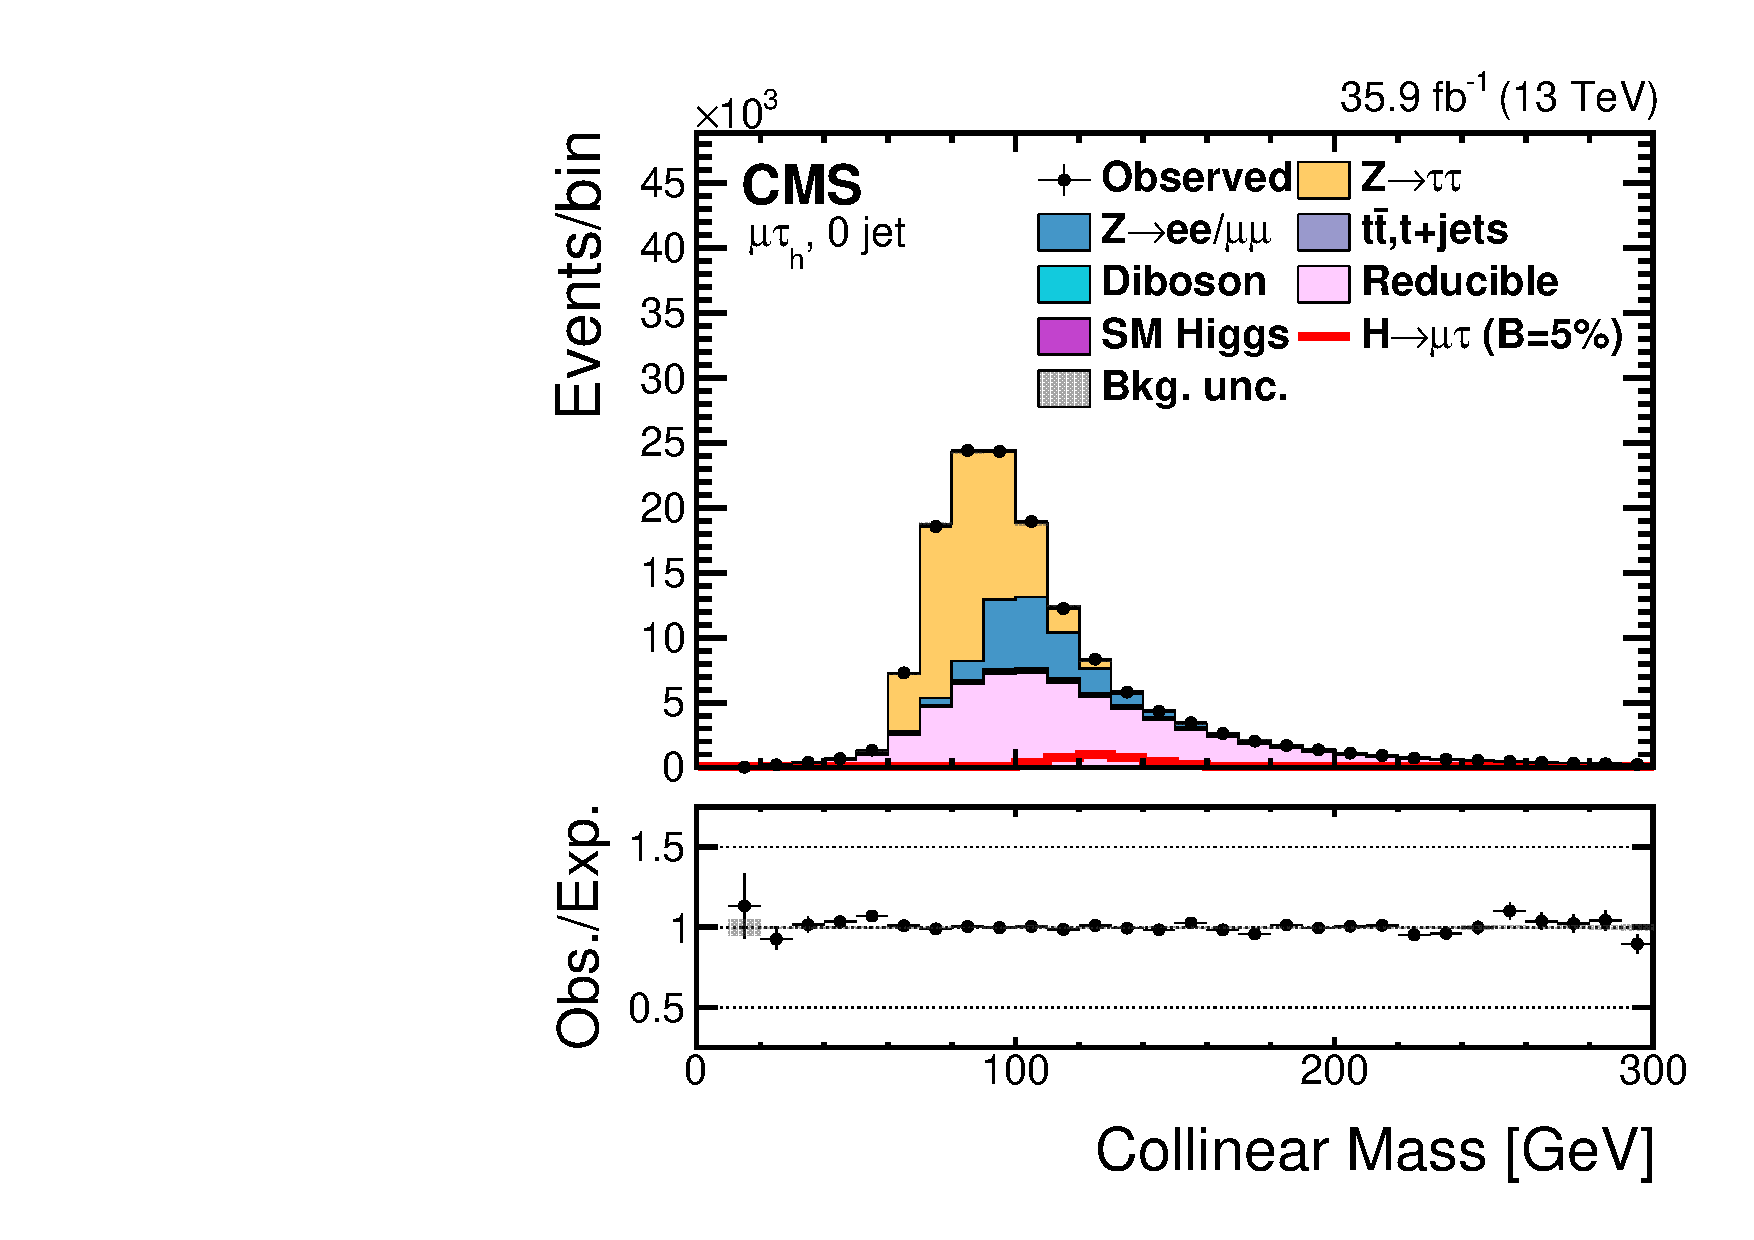
\includegraphics[width=0.4\textwidth]{chapter8/mutau_HMuTau_mutauhad_1_2016_postfit_COLMASS.pdf}}
     \caption[$\mcol$ distribution after the selection in $\Hmuhad$ analysis]{$\mcol$ distribution after the selection. The signal and backgrounds in the plots have been normalized to the best fit values. The gray bands shows the total uncertainties in each bin and the signal is plotted with the branching ratio of 5\% of the Higgs decay branching ratio for visualization purpose.}
     \label{fig:cutbasedpostfit}
\end{figure}


\begin{figure}[htbp] 
     \centering
     \subfigure[0 jet]{ 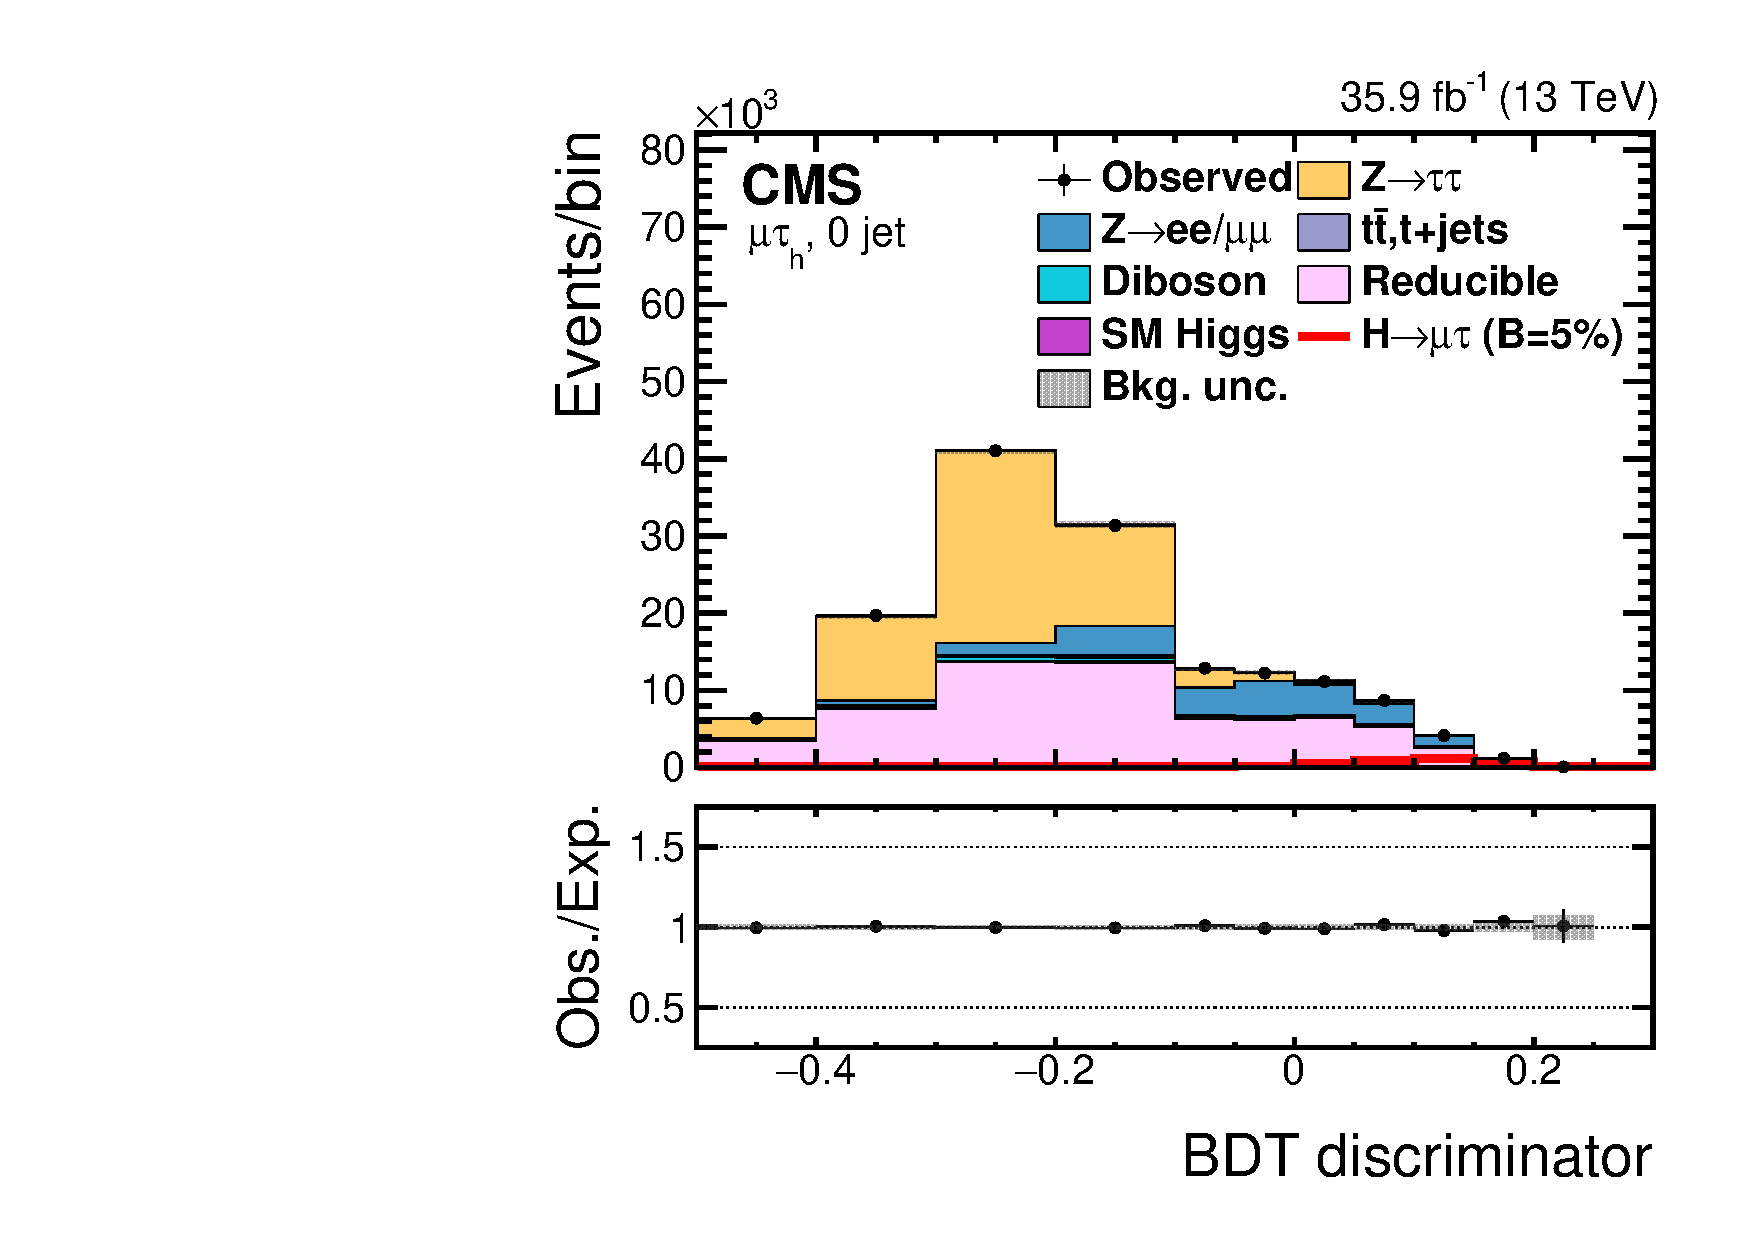
\includegraphics[width=0.4\textwidth]{chapter8/mutau_HMuTau_mutauhad_1_2016_postfit_BDT.pdf}}
     \subfigure[1 jet]{ 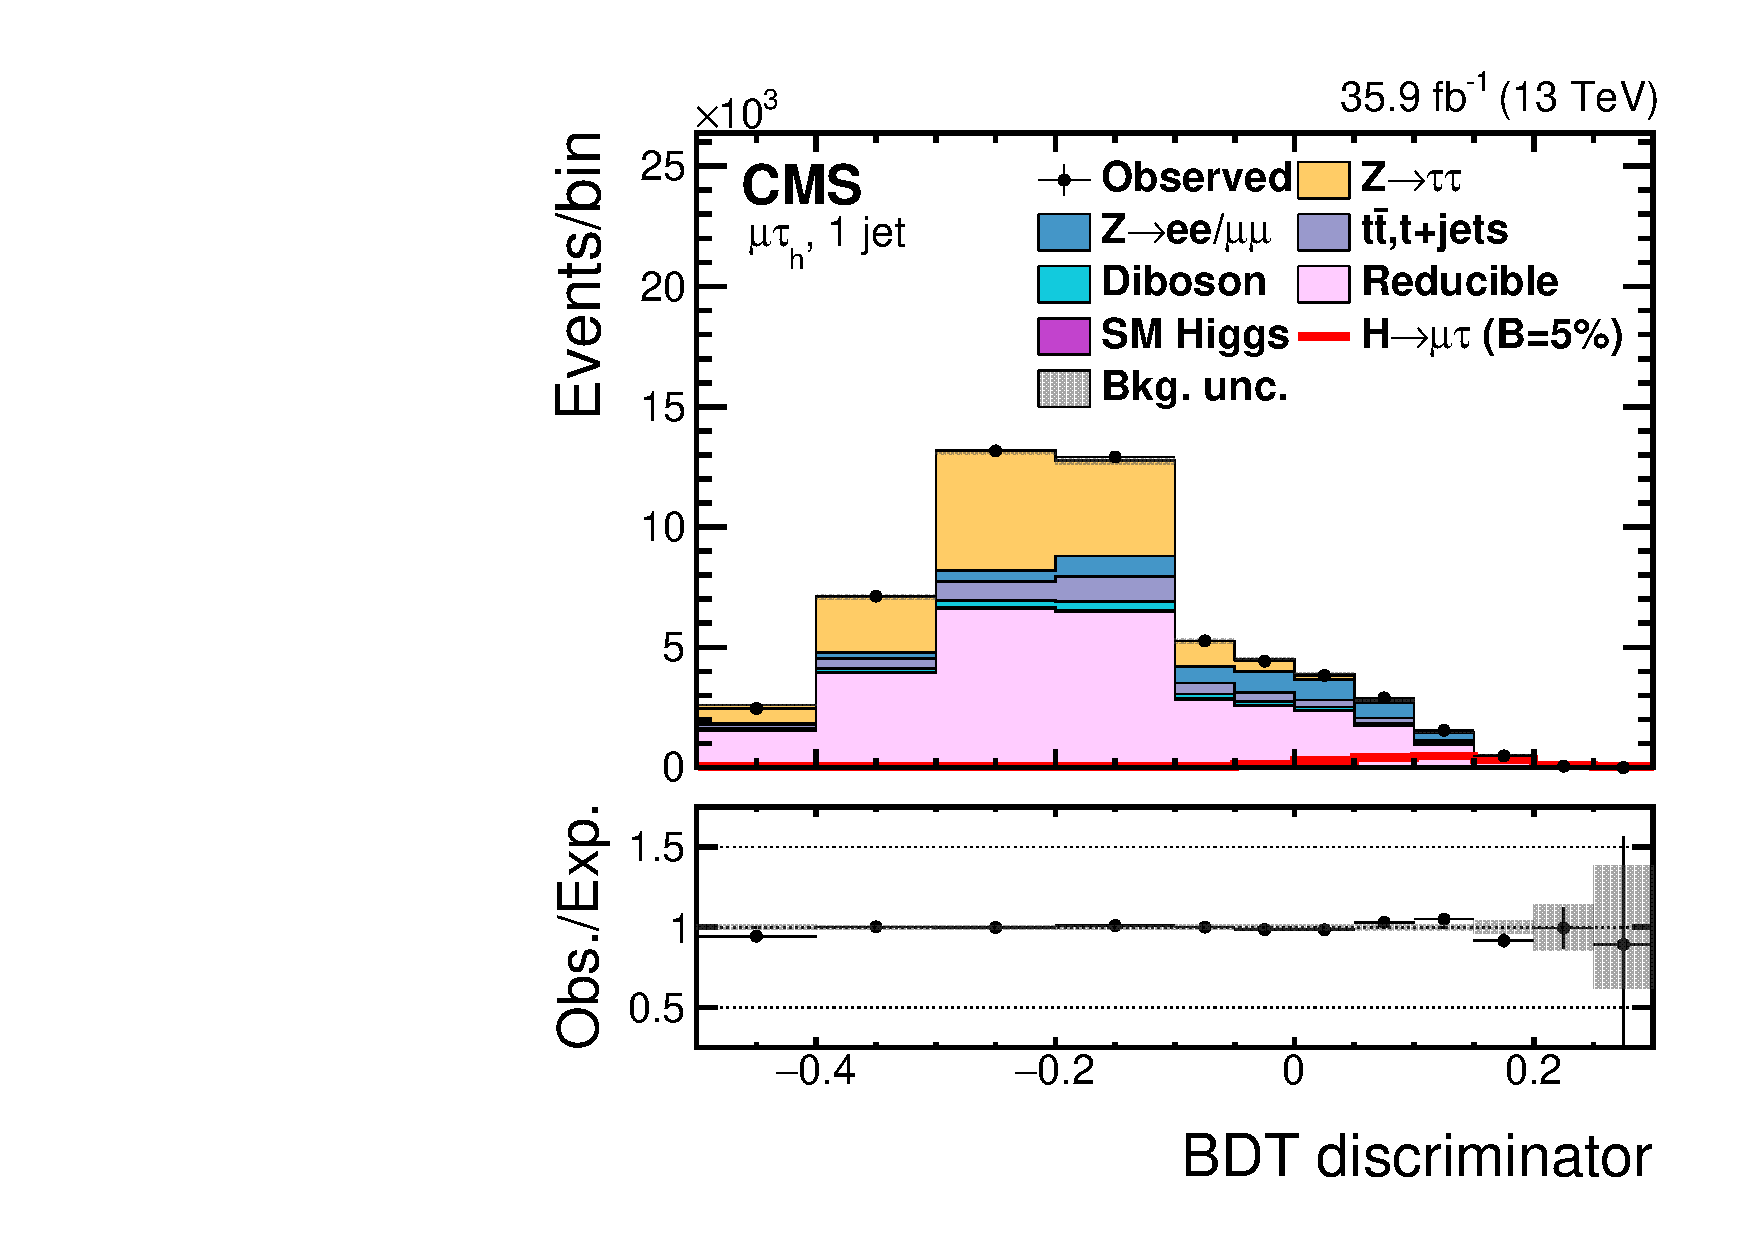
\includegraphics[width=0.4\textwidth]{chapter8/mutau_HMuTau_mutauhad_2_2016_postfit_BDT.pdf}}\\
     \subfigure[2 jets, gg-enriched]{ 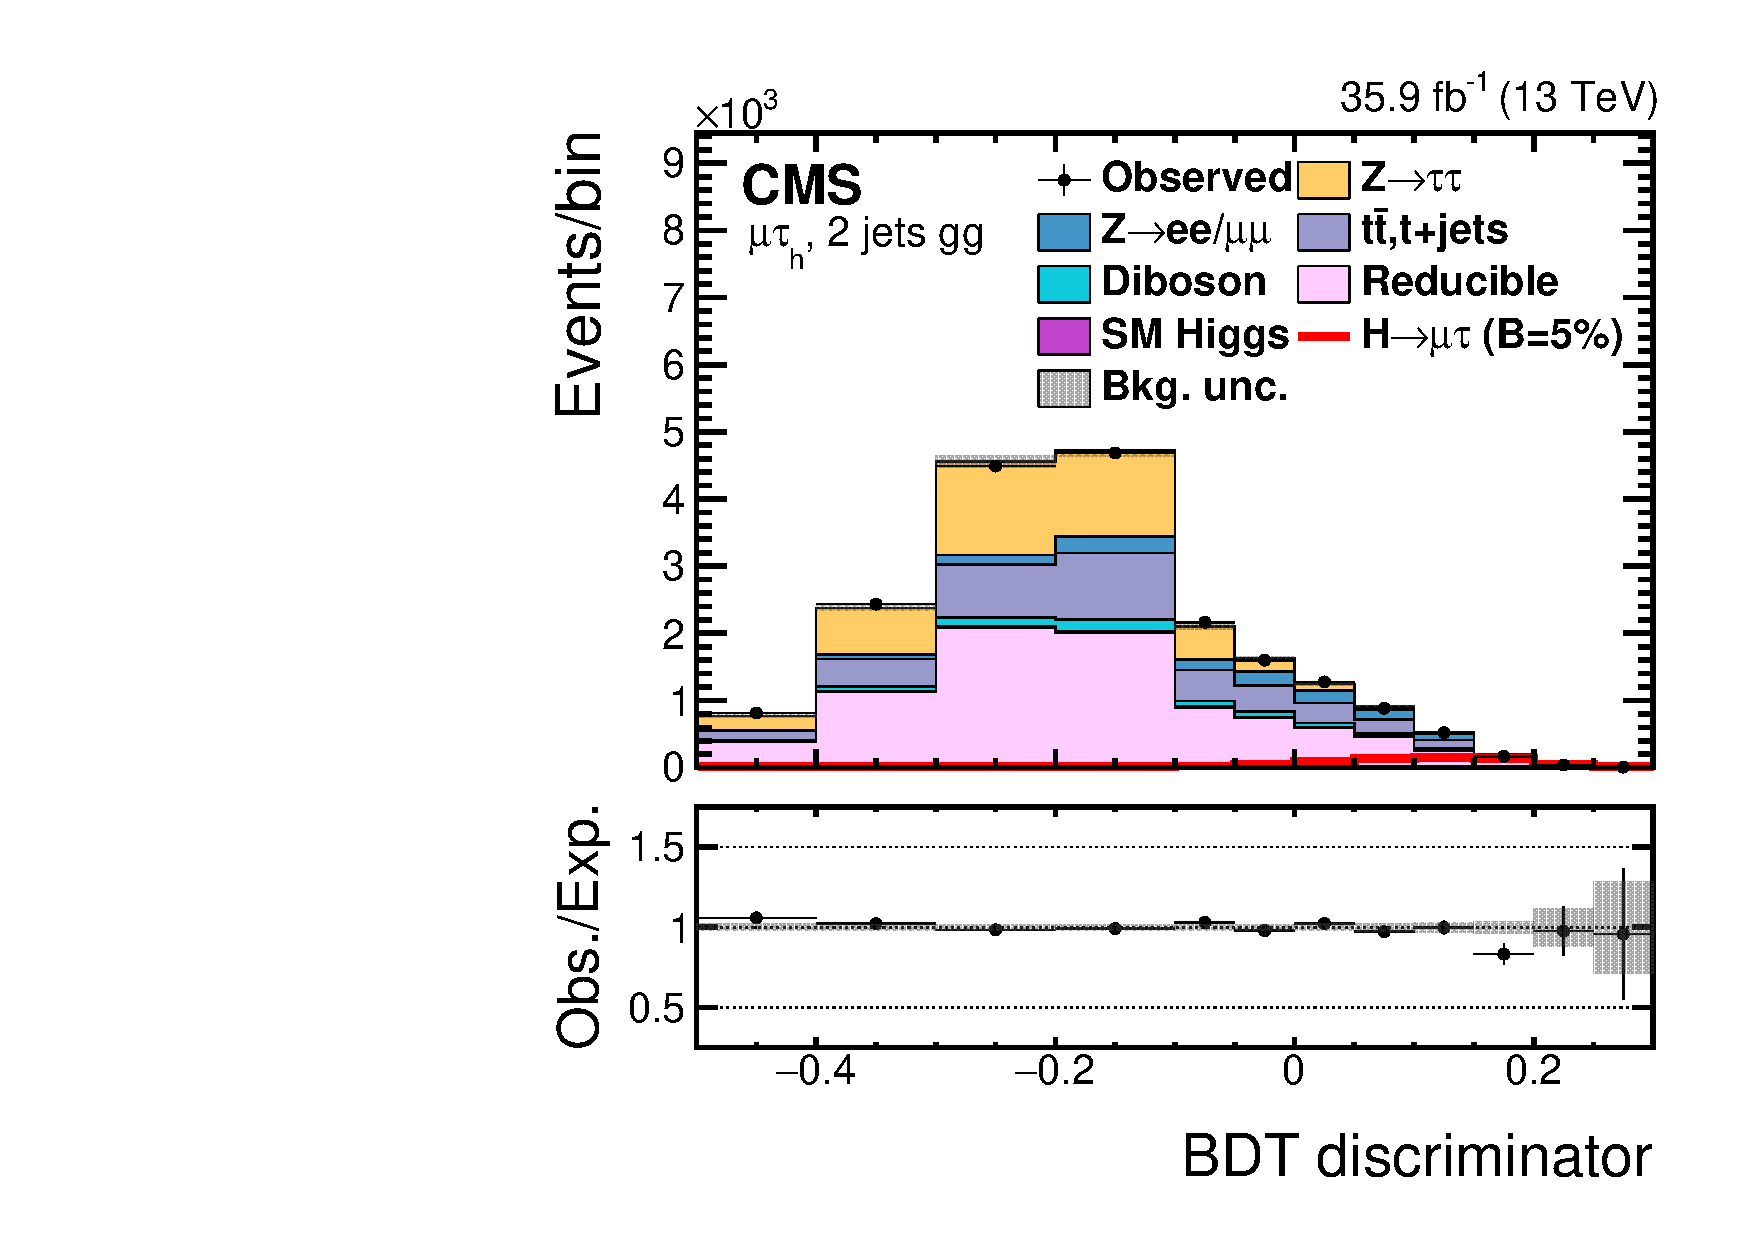
\includegraphics[width=0.4\textwidth]{chapter8/mutau_HMuTau_mutauhad_3_2016_postfit_BDT.pdf}}
     \subfigure[2 jets, VBF-enriched]{ 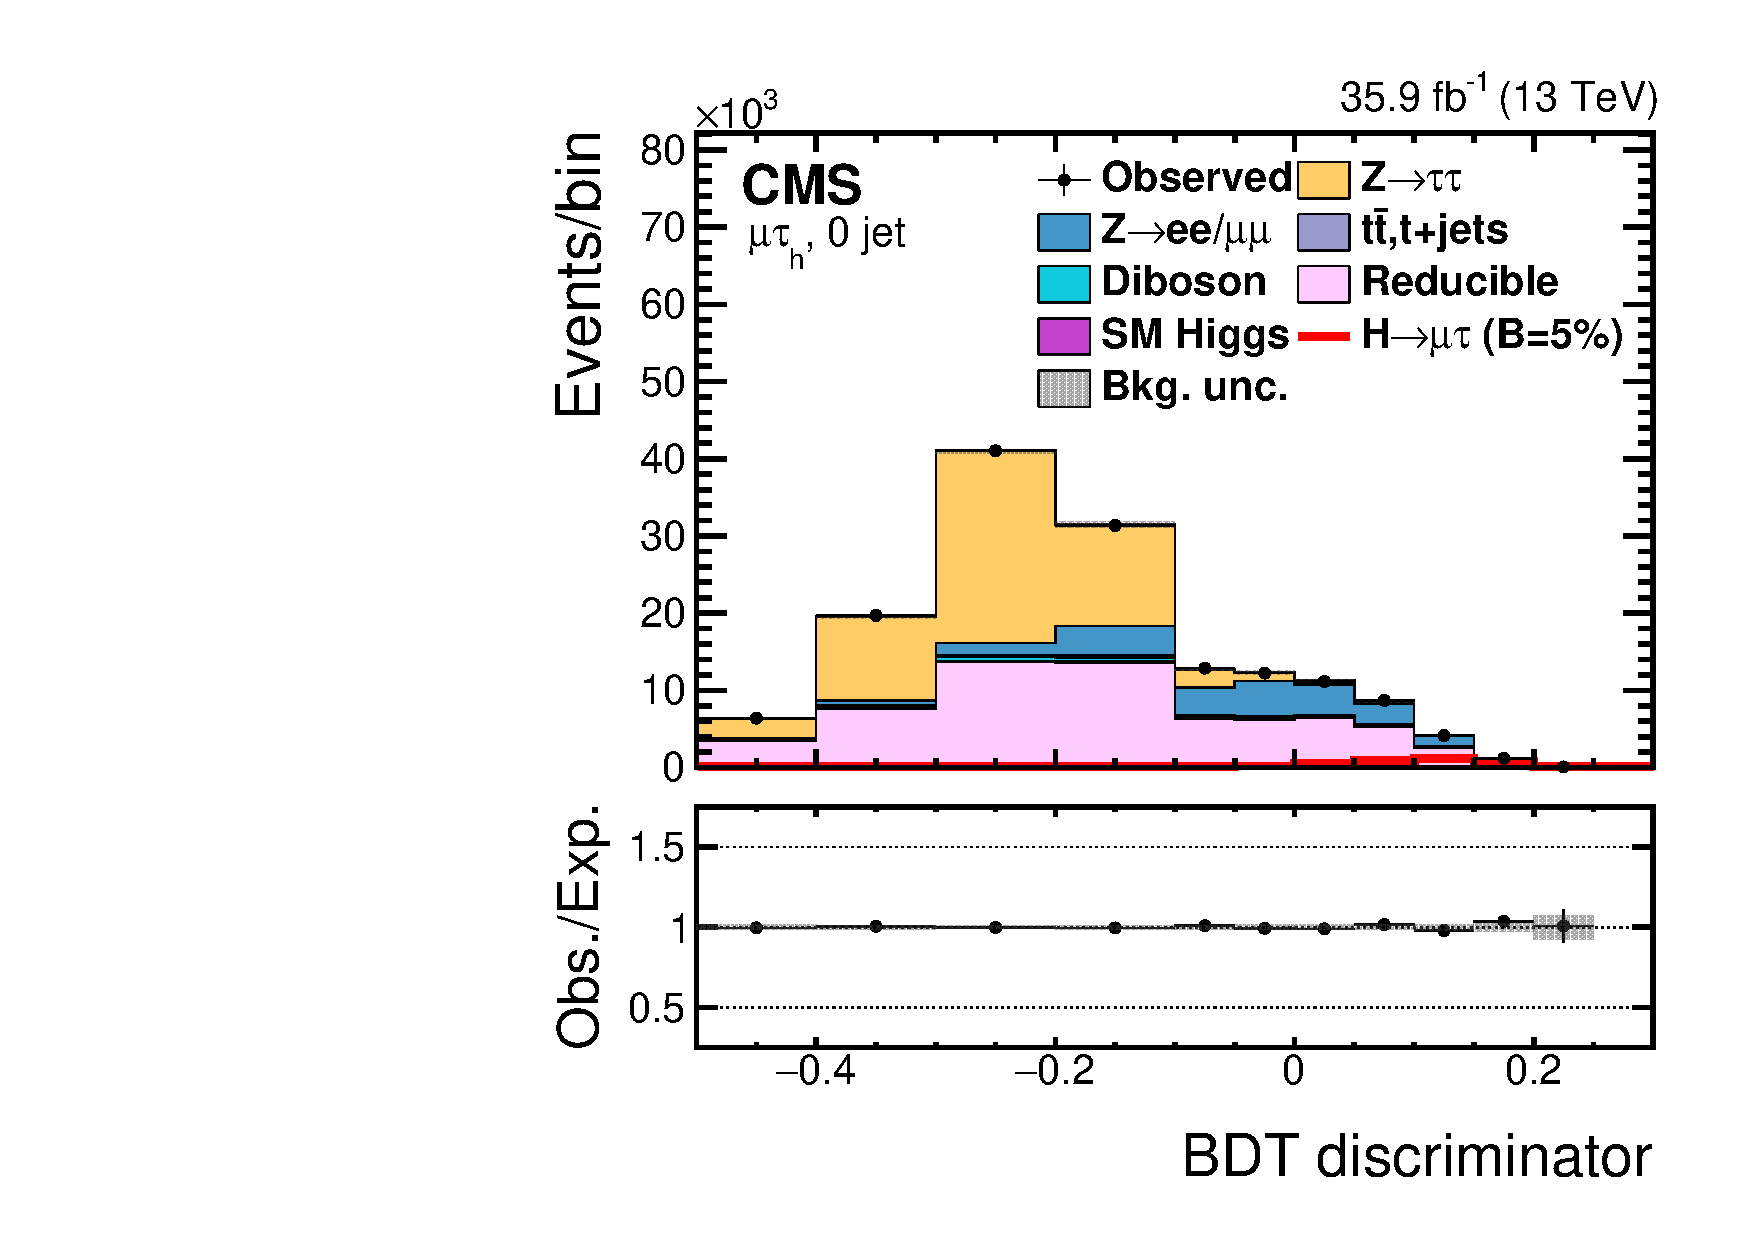
\includegraphics[width=0.4\textwidth]{chapter8/mutau_HMuTau_mutauhad_1_2016_postfit_BDT.pdf}}
     \caption[The BDT discriminator distribution of $\Hmuhad$ anlaysis]{The BDT discriminator distribution after the training. The signal and backgrounds in the plots has been normalized to the best fit values. The gray bands shows the total uncertainties in each bin and the signal is plotted with the branching ratio of 5\% of the Higgs decay branching ratio for visualization purpose. }
     \label{fig:bdtbasedpostfit}
\end{figure}


\begin{table}[!htpb]
 \centering
 \caption{$\mcol$ FIT ANALYSIS EXPECTED AND OBSERVED UPPER LIMITS AT 95\% CL AND THE BEST FIT BRANCHING FRACTIONS IN EACH OF THE CATEGORIES.}
 %  \caption{$\mcol$ fit analysis expected and observed upper limits at 95\% CL and the best fit branching fractions in each of the categories.}
 \label{tab:expected_limits_CutBased_MuTau}
\begin{tabular}{c|c|c|c|c|c}
  \noalign{\vskip 2mm}
   \hline
\multicolumn{6}{c}{Expected limits~(\%) } \\ \hline
                       &  \multicolumn{1}{c|}{0-jet}   & \multicolumn{1}{c|}{1-jet}    &  \multicolumn{1}{c|}{2-jets} & \multicolumn{1}{c|}{VBF}  & \multicolumn{1}{c}{Combined}                 \\  \cline{2-6}
%$\mu\tau_{\textrm{e}}$   &  $<$ 1.01     &  $<$ 1.47     &  $<$ 3.23     &  $<$ 1.73     &  $<$ 0.75    \\
$\mu\tau_{h}$    &  $<$ 1.14     &  $<$ 1.26     &  $<$ 2.12     &  $<$ 1.41     &  $<$ 0.71    \\
%\cline{2-6}
% $\mu\tau$  & \multicolumn{5}{c}{ $<$ 0.49  } \\ \hline
  \noalign{\vskip 2mm}
            \hline

\multicolumn{6}{c}{Observed limits~(\%)} \\ \hline
                       &  \multicolumn{1}{c|}{0-jet}   & \multicolumn{1}{c|}{1-jet}    &  \multicolumn{1}{c|}{2-jets} & \multicolumn{1}{c|}{VBF}  & \multicolumn{1}{c}{Combined}                 \\  \cline{2-6}
%$\mu\tau_{\textrm{e}}$                   & $<$ 1.08      & $<$ 1.35      & $<$ 3.33      & $<$ 1.40      & $<$ 0.71    \\
$\mu\tau_{h}$                    & $<$ 1.04      & $<$ 1.74      & $<$ 1.65      & $<$ 1.30      & $<$ 0.66    \\
%\cline{2-6}
 % $\mu\tau$  & \multicolumn{5}{c}{ $<$ 0.51  } \\ \hline

  \noalign{\vskip 2mm}
            \hline
\multicolumn{6}{c}{Best fit branching fractions~(\%)} \\ \hline
                       &  \multicolumn{1}{c|}{0-jet}   & \multicolumn{1}{c|}{1-jet}    &  \multicolumn{1}{c|}{2-jets} & \multicolumn{1}{c|}{VBF} &\multicolumn{1}{c}{Combined}                 \\  \cline{2-6}
%$\mu\tau_{\textrm{e}}$                   & 0.13 $\pm$ 0.43       & -0.22 $\pm$ 0.75      & 0.22 $\pm$ 1.39       & -1.73 $\pm$ 1.05      & -0.04 $\pm$ 0.33  \\
$\mu\tau_{h}$                    & -0.30 $\pm$ 0.45      & 0.68 $\pm$ 0.56       & -1.23 $\pm$ 1.04      & -0.23 $\pm$ 0.66      & -0.08 $\pm$ 0.34  \\
\hline
%\cline{2-6}
% $\mu\tau$  & \multicolumn{5}{c}{ 0.02 $\pm$ 0.20 } \\ \hline
\end{tabular}
\end{table}


\begin{table}[!htpb]
 \centering
 \caption{BDT FIT ANALYSIS EXPECTED AND OBSERVED UPPER LIMITS AT 95\% CL AND THE BEST FIT BRANCHING FRACTIONS IN EACH OF THE CATEGORIES.}
 % \caption{BDT fit analysis expected and observed upper limits at 95\% CL and the best fit branching fractions in each of the categories.}
 \label{tab:expected_limits_BDTMethod2_MuTau}
\begin{tabular}{*{6}{c}}
\multicolumn{6}{c}{Expected limits~(\%) } \\ \hline
                       &  \multicolumn{1}{c}{0-jet}   & \multicolumn{1}{c}{1-jet}    &  \multicolumn{1}{c}{2-jets} & \multicolumn{1}{c}{VBF}  & \multicolumn{1}{c}{Combined}                 \\  \cline{2-6}
%$\mu\tau_{e}$         &  $<$0.83      &  $<$1.19      &  $<$1.98      &  $<$1.62      &  $<$0.59    \\
$\mu\tau_{h}$      &  $<$0.43      &  $<$0.56      &  $<$0.94      &  $<$0.58      &  $<$0.29    \\
%\cline{2-6}
% $\mu\tau$  & \multicolumn{5}{c}{ $<$0.25  }\\
\multicolumn{6}{c}{Observed limits~(\%)} \\ \hline
                       &  \multicolumn{1}{c}{0-jet}   & \multicolumn{1}{c}{1-jet}    &  \multicolumn{1}{c}{2-jets} & \multicolumn{1}{c}{VBF} &\multicolumn{1}{c}{Combined}                 \\ \cline{2-6}
%$\mu\tau_{e}$                 & $<$1.30       & $<$1.34       & $<$2.27       & $<$1.79       & $<$0.86    \\
$\mu\tau_{h}$              & $<$0.51       & $<$0.53       & $<$0.56       & $<$0.51       & $<$0.27    \\
%\cline{2-6}
 %$\mu\tau$  & \multicolumn{5}{c}{ $<$0.25  } \\
\multicolumn{6}{c}{Best fit branching fractions~(\%)} \\ \hline
                       &  \multicolumn{1}{c}{0-jet}   & \multicolumn{1}{c}{1-jet}    &  \multicolumn{1}{c}{2-jets} & \multicolumn{1}{c}{VBF} &\multicolumn{1}{c}{Combined}                 \\  \cline{2-6}
%$\mu \tau_{e}$                 & 0.61 $\pm$ 0.36       & 0.22 $\pm$ 0.46       & 0.39 $\pm$ 0.83       & 0.10 $\pm$ 1.37       & 0.35 $\pm$ 0.26  \\
$\mu\tau_{h}$              & 0.12 $\pm$ 0.20       & $-0.05$ $\pm$ 0.25    & $-0.72$ $\pm$ 0.43    & $-0.22$ $\pm$ 0.31    & $-0.04$ $\pm$ 0.14  \\  \hline
%\cline{2-6}
 %$\tau\tau$  & \multicolumn{5}{c}{ 0.00 $\pm$ 0.12 } \\ \hline
  \end{tabular}
\end{table}


\begin{figure}[htbp] 
     \centering
     \subfigure[$\mcol$ fit analysis]{ 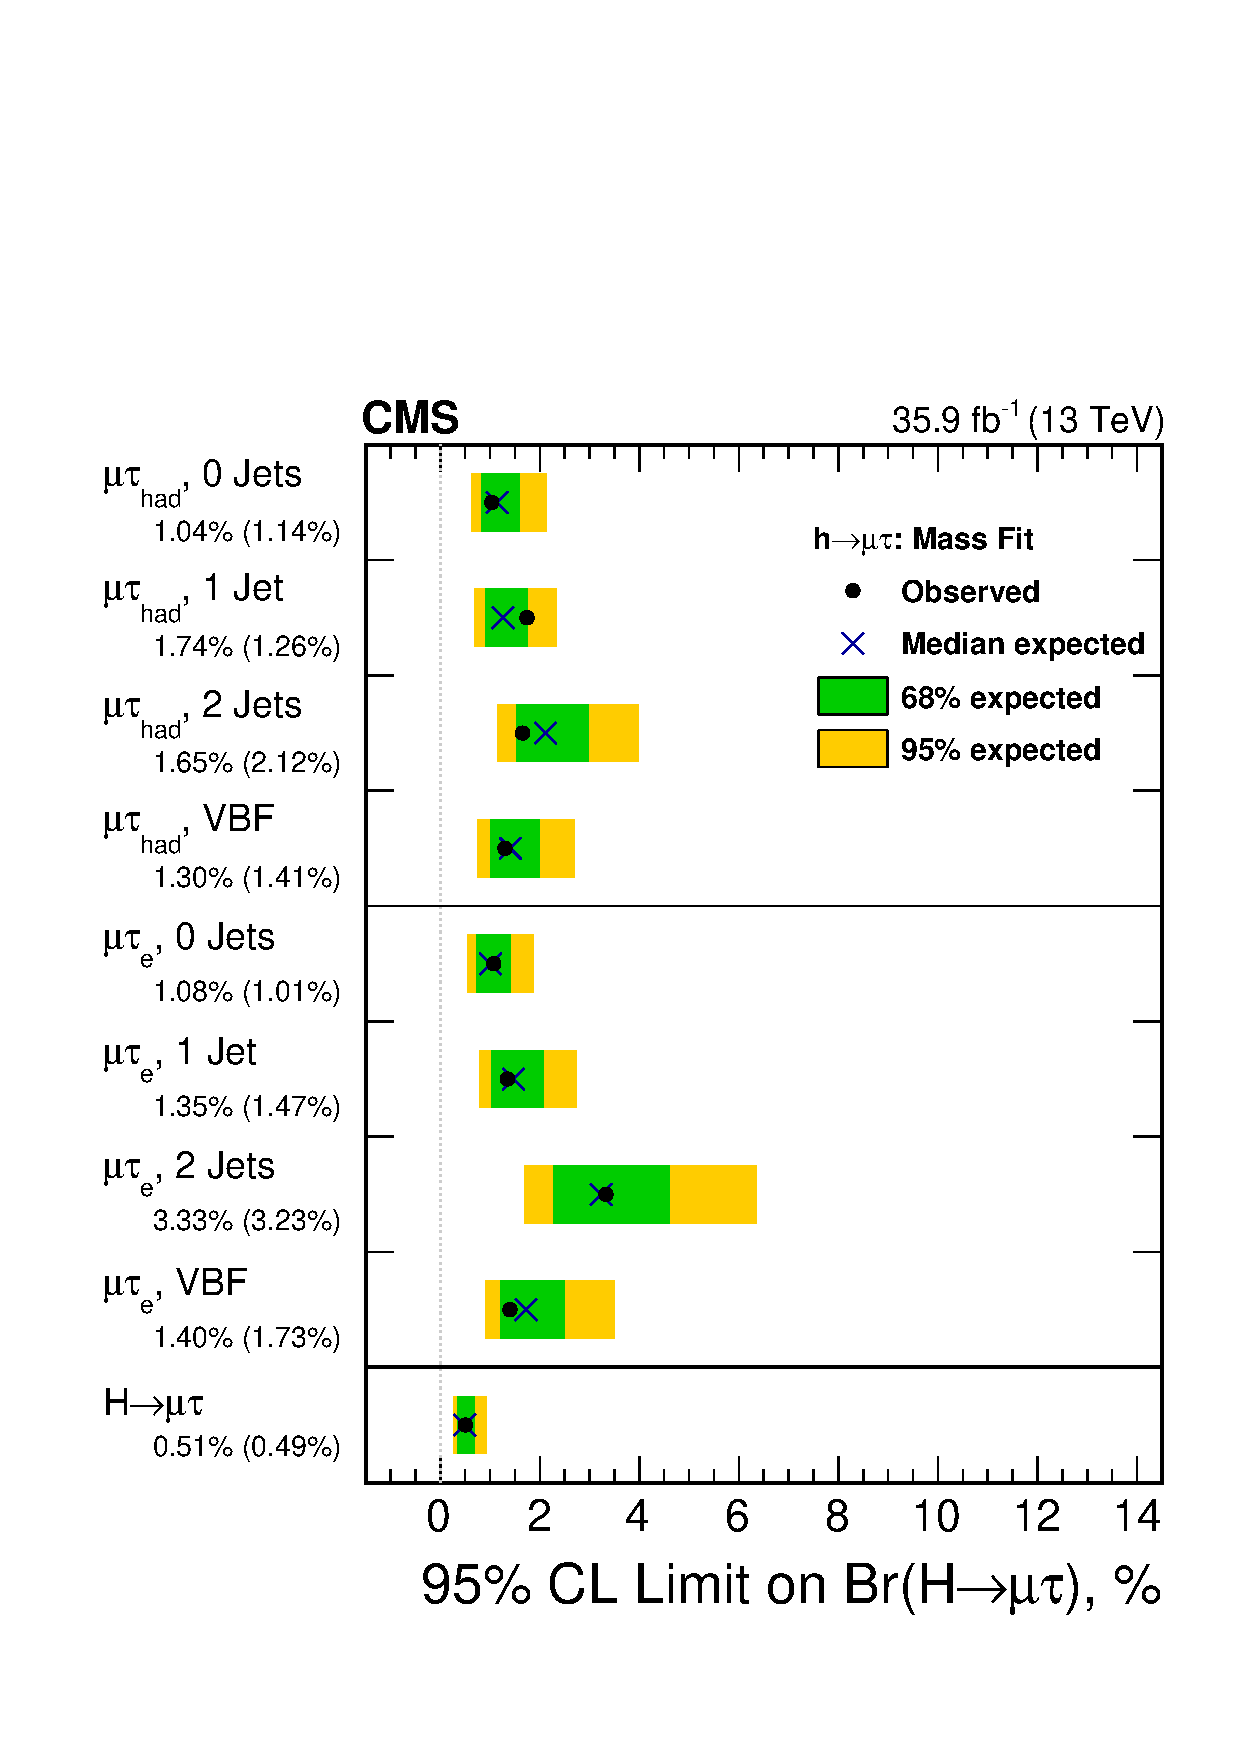
\includegraphics[width=0.4\textwidth]{chapter8/HMUTAU_CB_SUMMARY.pdf}}
     \subfigure[BDT fit analysis]{ 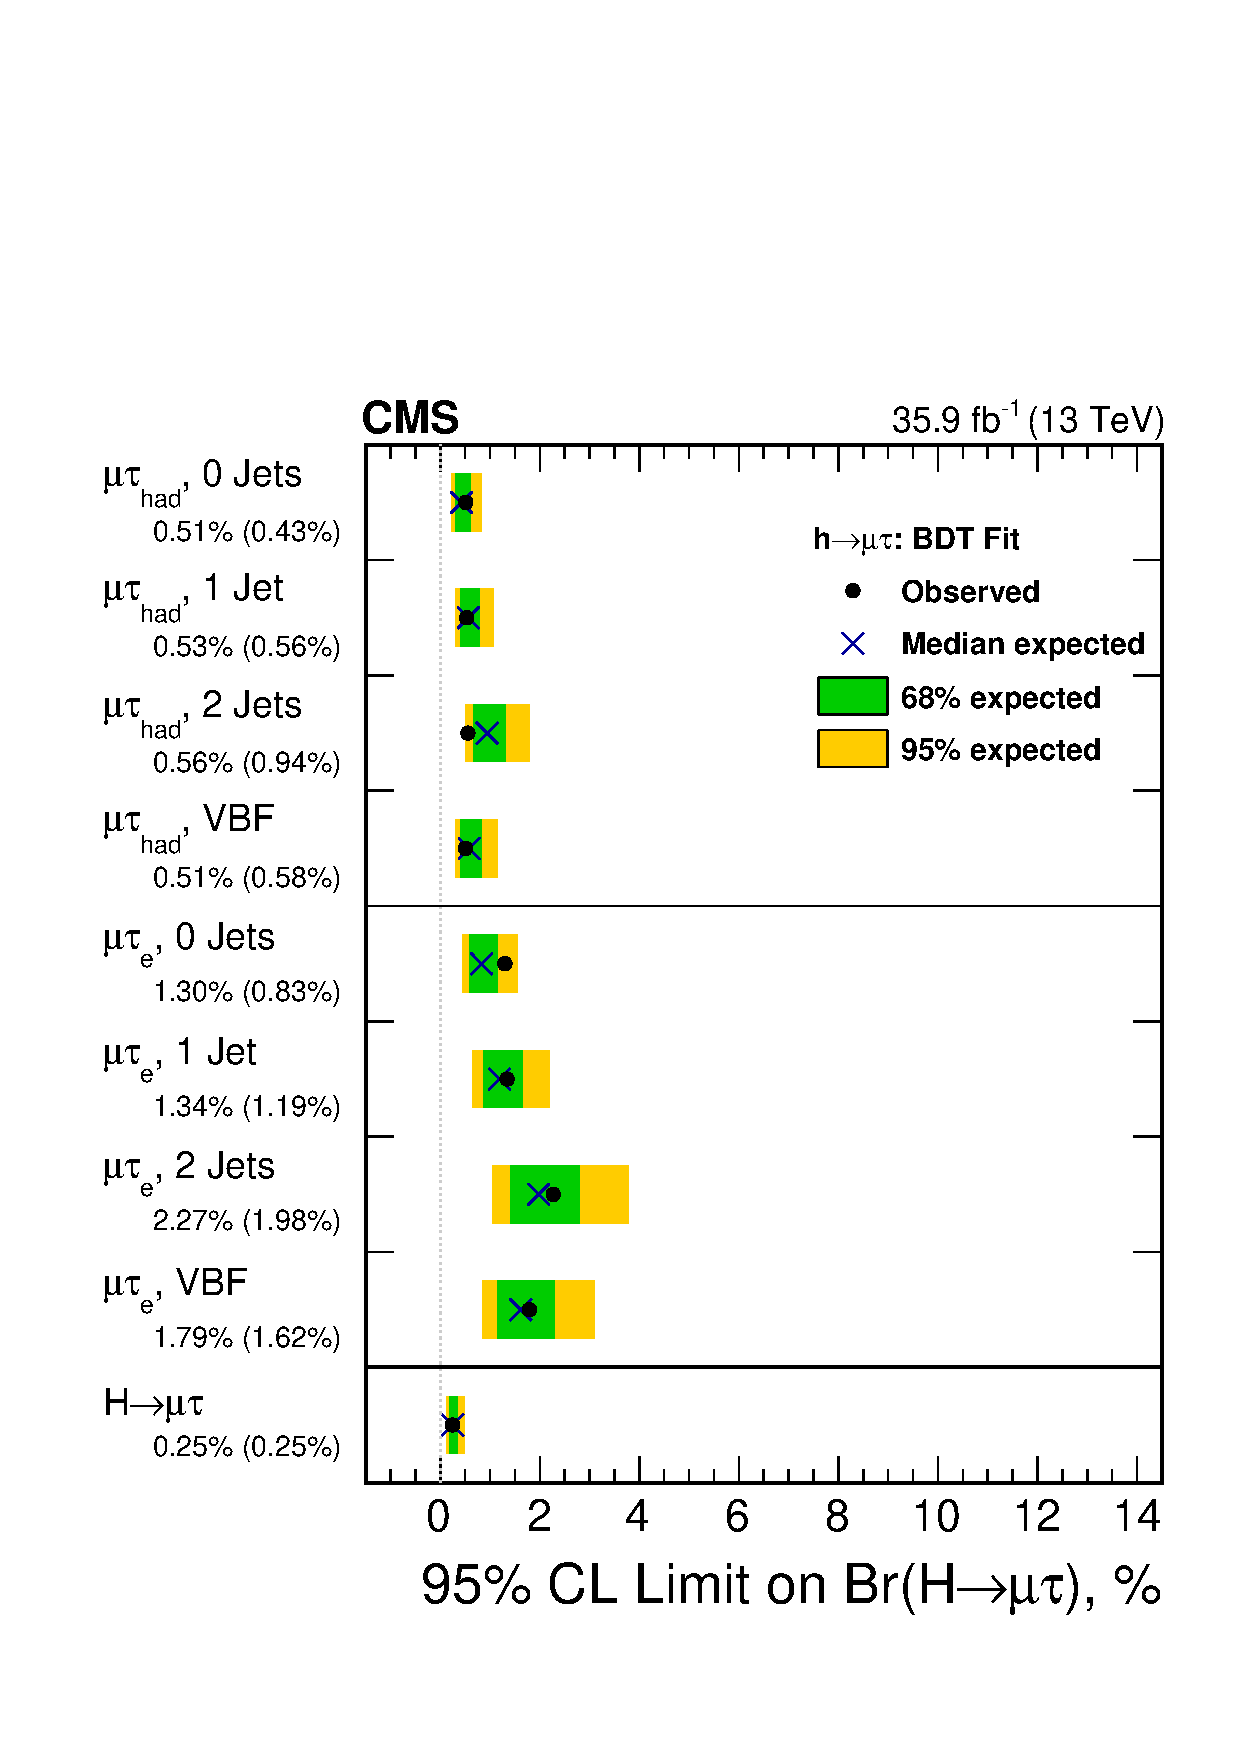
\includegraphics[width=0.4\textwidth]{chapter8/HMUTAU_BDT_SUMMARY.pdf}}\\
     \caption[The expected and observed limits on $H \to \mu \tau$ analysis]{The expected and observed 95\% CL limits on branching ratio of total $H \to \mu\tau$ which shows the results from both $\Hmuhad$ and $H \to \mu\tau_{e}$ in the $\mcol$ fit analysis and BDT fit analysis.}
     \label{fig:cutbasedpostfit}
\end{figure}




\begin{figure}[htpb]
\begin{center}
\includegraphics[width=0.6\textwidth]{chapter8/yukawaMuon_dark.pdf}
\end{center}
\caption[Upper limit of flavour violating Yukawa coupling  from the $H \to \mu\tau$ BDT fit analysis]{Upper limit of flavour violating Yukawa coupling $|Y_{\mu\tau}|, |Y_{\tau\mu}|$ from the BDT fit analysis. The red solid line represents the expected limit and the black solid line is the observed limit. 68\% and 95\% range of containing the observed limit is shown in the green and yellow band. The result from $\tau \to 3 \mu$ is shown in dark green~\cite{Hayasaka:2010np,Olive:2016xmw,Harnik:2012pb} and the one from $\tau \to \mu\gamma$ is shown in lighter green~\cite{Olive:2016xmw,Harnik:2012pb}. The theoretical naturalness limit $Y_{ij}Y_{ji} \leq m_im_j/v^2$ is shown by purple diagonal line~\cite{Harnik:2012pb}.}

\label{fig:Yukawas}
\end{figure}






\subsection{Results in $\Hehad$ search}
The search of $\Hehad$ is performed in $\mcol$ fit analysis with CMS 8 TeV 19.7 $fb^{-1}$. The analysis is binned with 3 categories. After applying the selection cuts and adjusting the signal and background processes by the fit, the fitting variable $\mcol$ distribution is shown in Figure.~\ref{fig:etaubdtbasedpostfit}. The number of event yields of both signal and background processes are shown in Table.~\ref{tab:EventYieldTable_100_to_150}. The yields are normalized to the integrated luminosity of 19.7 $fb^{-1}$ and the signal branching ratio is assumed to be 0.69\% of the SM Higgs production cross section. This thesis is focused and written on the analysis $\Hehad$ which is one part of the whole search on lepton flavour violating Higgs decay to $e\tau$. Another closely related search is $\Hetaumu$~\cite{HIG-14-040}. The results of each categories and combined ones of the two analysis $\Hehad$ and $\Hetaumu$ on the expected and observed upper signal branching fraction $\mathcal{B}(H \to e \tau)$ limits is shown in Table.~\ref{tab:expected_limits} and summarized in Figure.~\ref{fig:Etaulimitsummary}.  The combined upper limit on $\mathcal{B}(H \to e \tau)<0.69$ is the first direct search on this channel and the tightest limit by the time the result was published. The Yukawa coupling between electron and tau leptons is related to decay width $\Gamma$ and branching fraction $\mathcal{B}$ as shown in Equation.~\ref{eq:Yukawa} and \ref{eq:Branchingfraction}. The 95\% CL upper limit on Yukawa coupling from the combined result in $\Het$ is $\sqrt{Y_{e\tau}|^2 + |Y_{\tau e}|^2}<2.4\times 10^{-3}$. The limit on $e\tau$ Yukawa coupling from this search and other previous search results are shown in Figure.~\ref{fig:etauYukawa}.









\begin{figure}[htbp] 
     \centering
     \subfigure[0 jet]{ 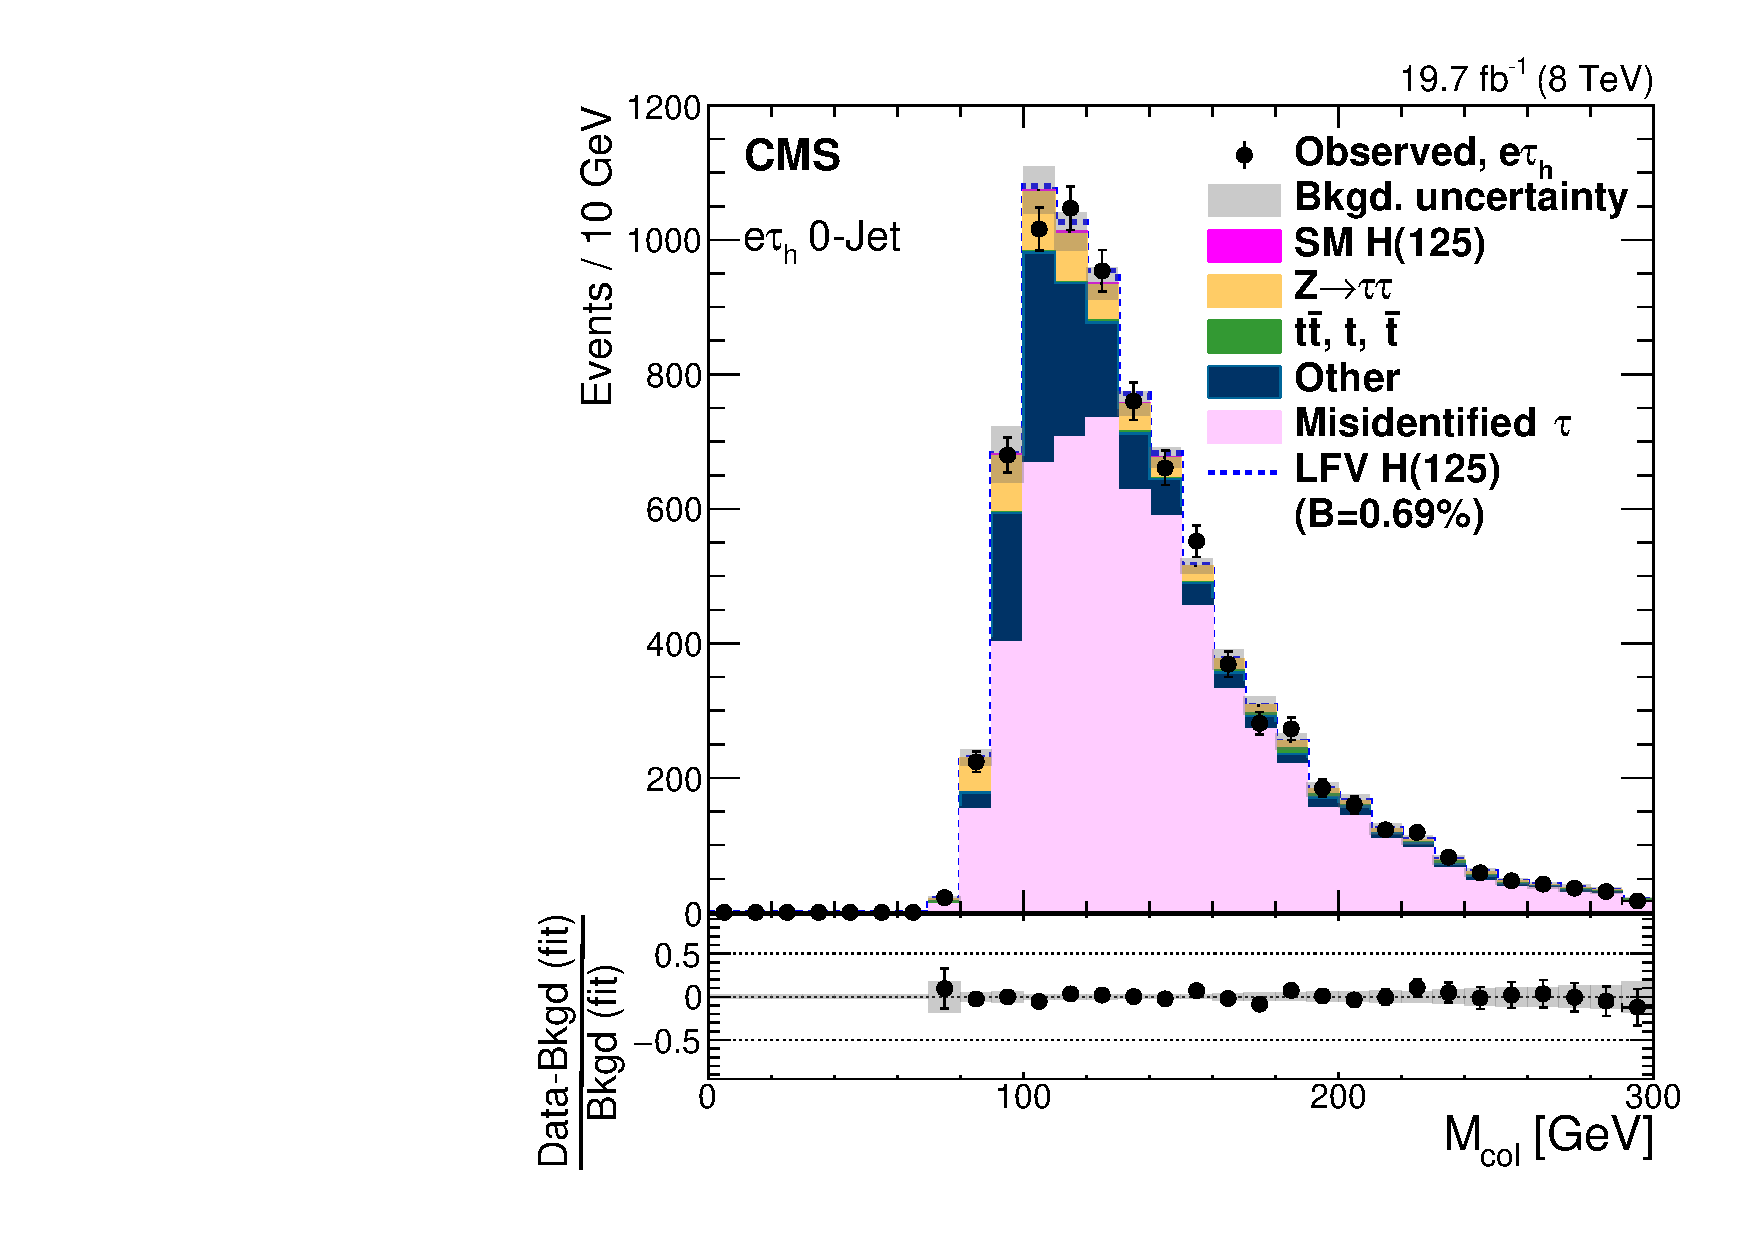
\includegraphics[width=0.4\textwidth]{chapter8/etau_HETau_etauhad_1_2016_postfit.pdf}}
     \subfigure[1 jet]{ 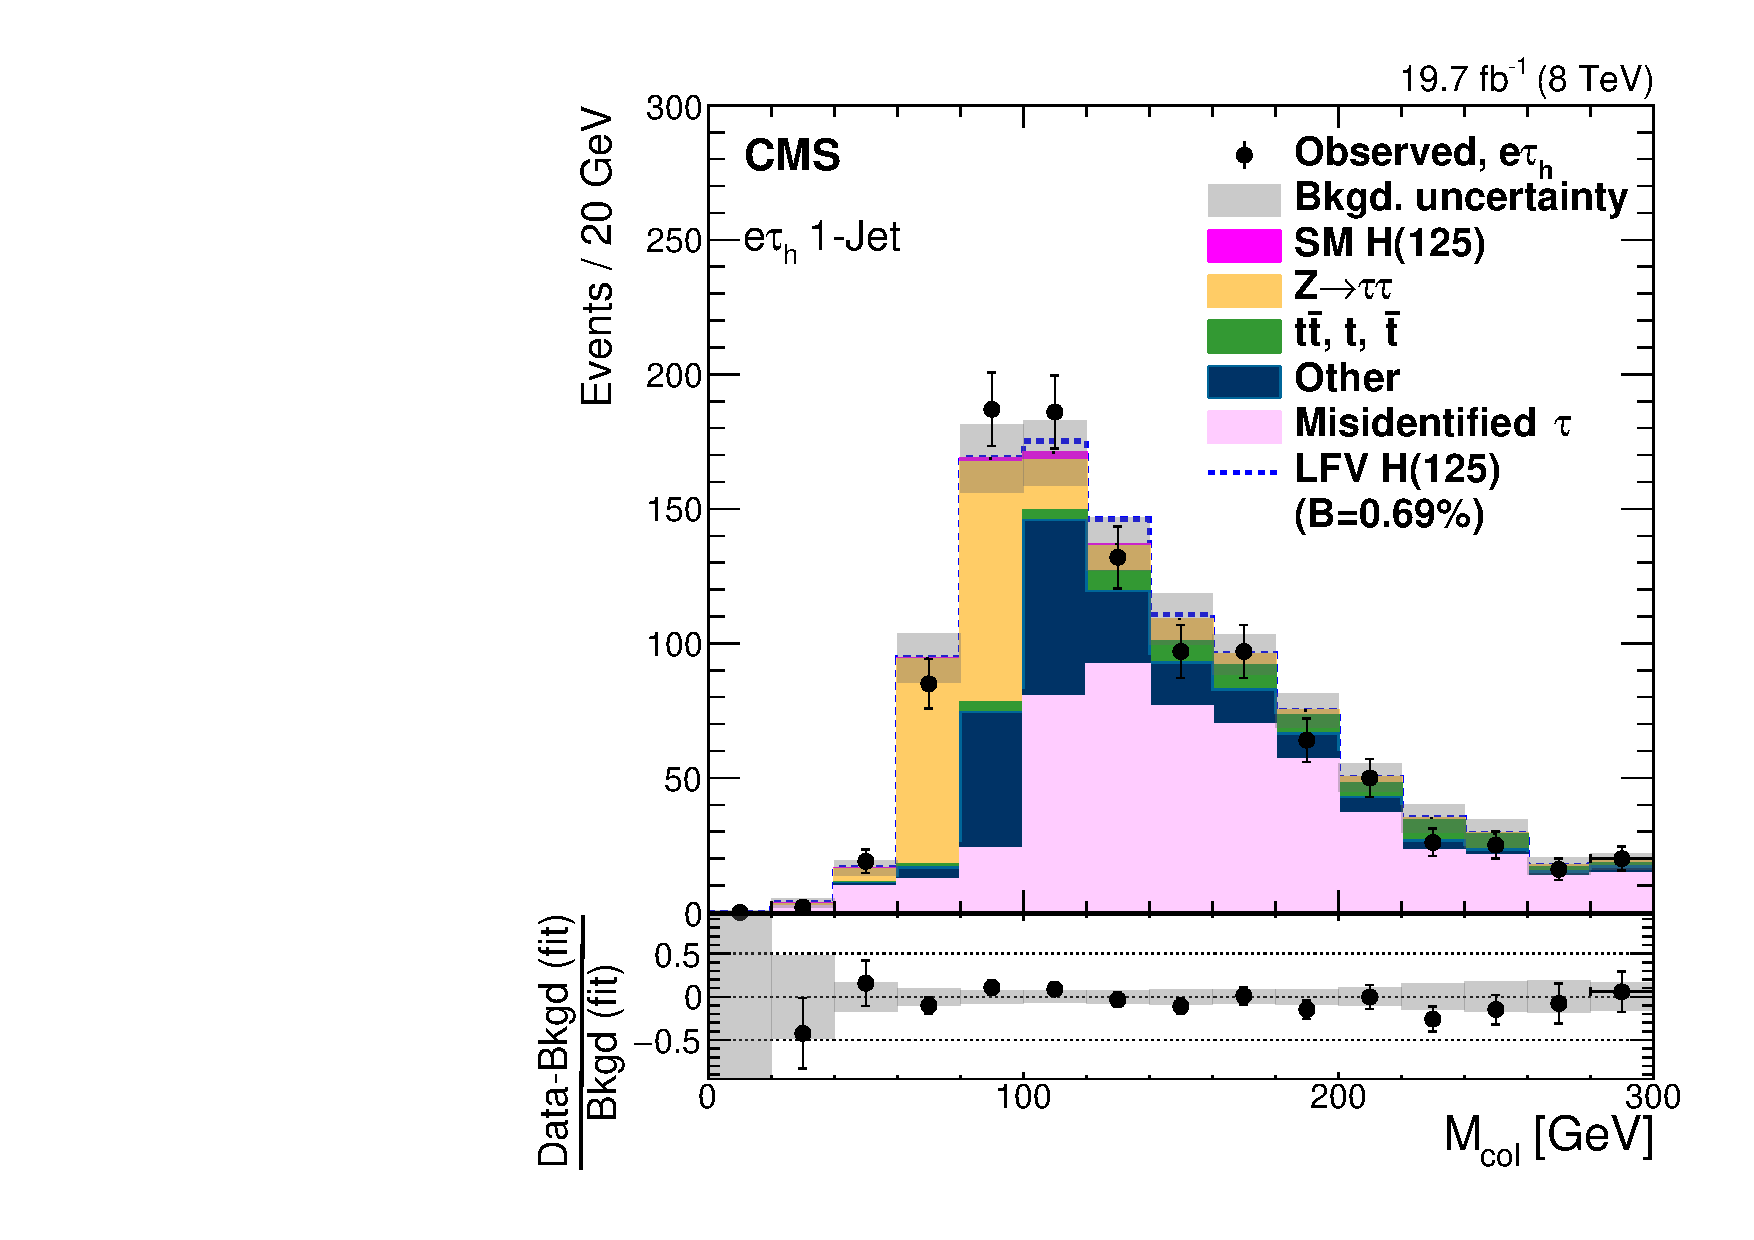
\includegraphics[width=0.4\textwidth]{chapter8/etau_HETau_etauhad_2_2016_postfit.pdf}}\\
     \subfigure[2 jets]{ 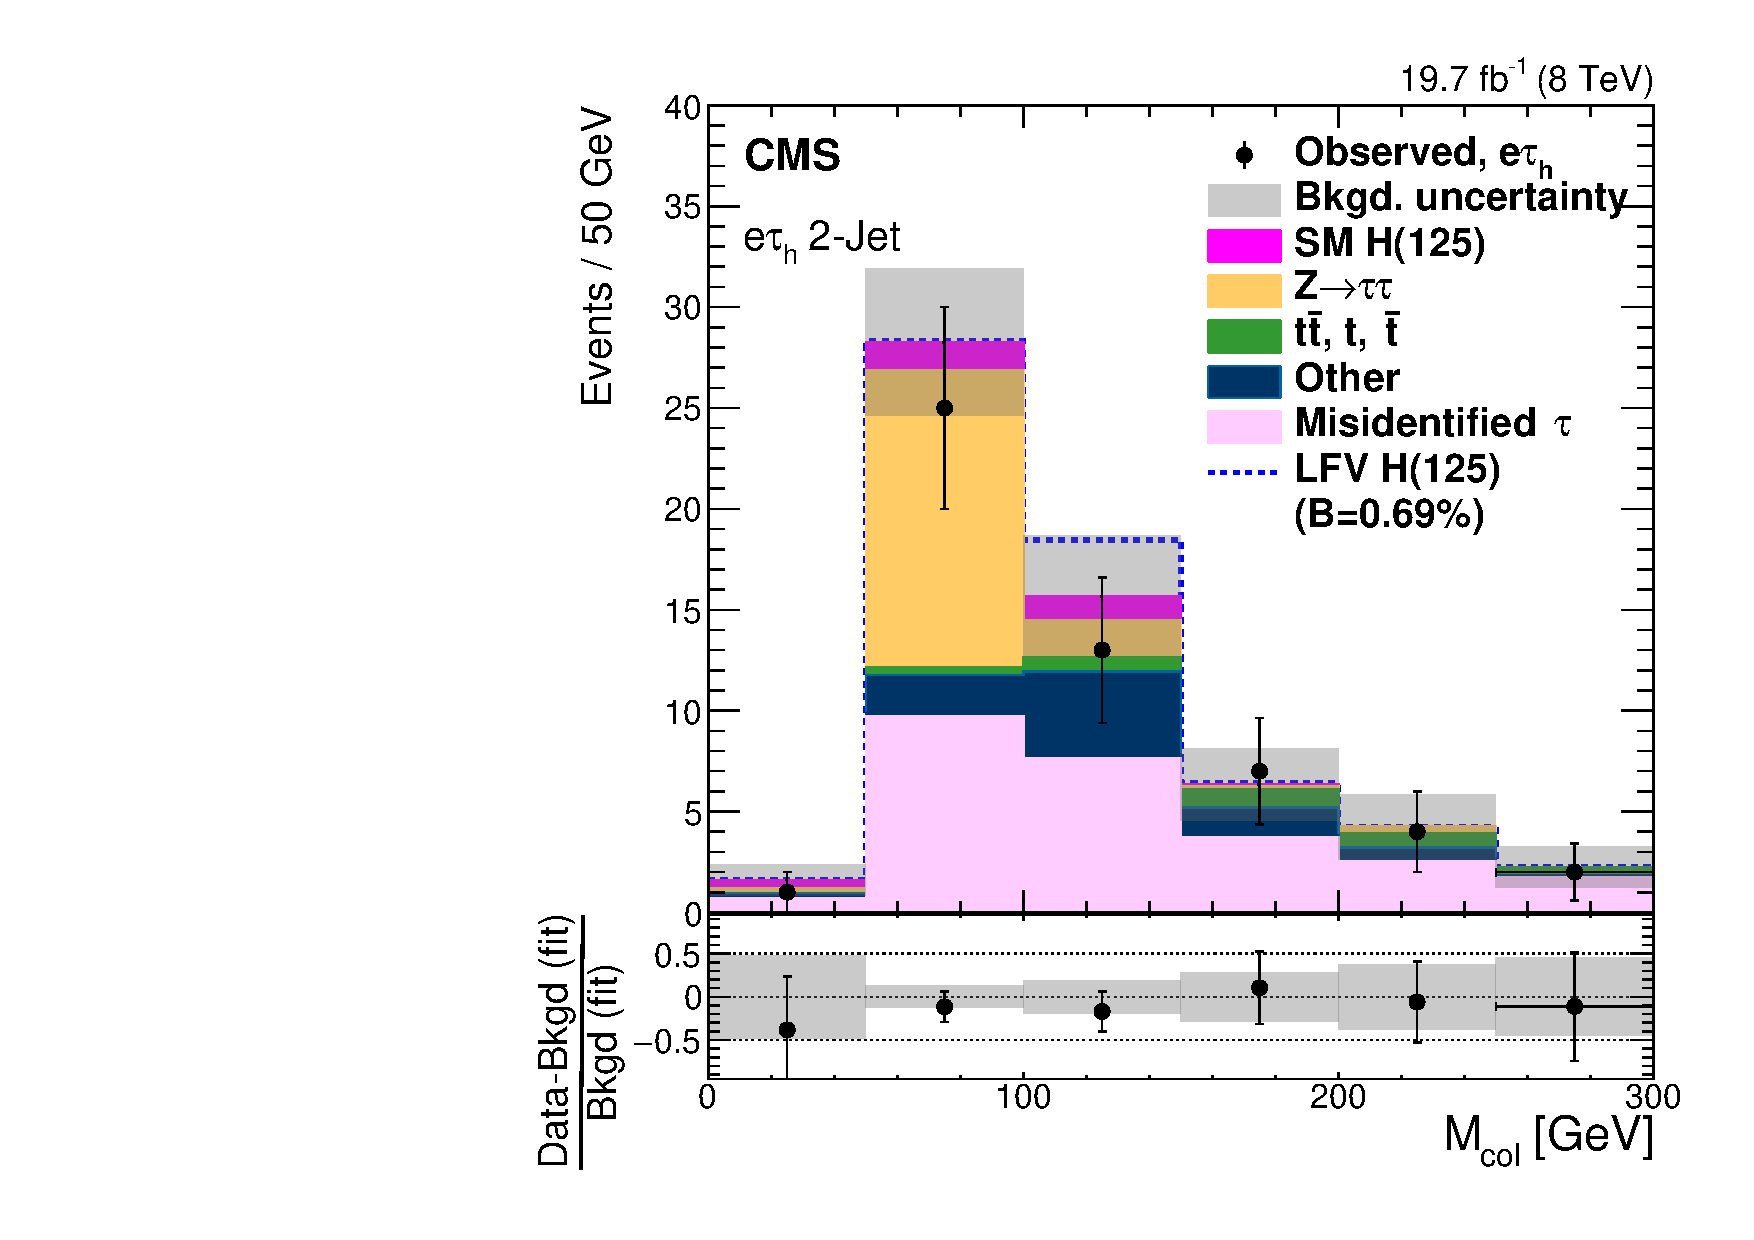
\includegraphics[width=0.4\textwidth]{chapter8/etau_HETau_etauhad_3_2016_postfit.pdf}}
     \caption[$\mcol$ distribution after the selection in $\Hehad$ analysis]{ $\mcol$ distribution after the selection. The signal and backgrounds in the plots have been normalized to the best fit values. The gray bands shows the total uncertainties in each bin and the signal is plotted with the branching ratio of 0.69\% of the Higgs decay branching ratio for visualization purpose. }
     \label{fig:etaubdtbasedpostfit}
\end{figure}



\begin{table}[htbp]
\centering
\caption{EVENTS YIELDS OF THE SIGNAL AND BACKGROUNDS IN THE $\Hehad$ ANALYSIS}\label{tab:EventYieldTable_100_to_150} 
\begin{threeparttable}
%\caption[Events yields of the signal and backgrounds are in $\Hehad$ analysis]{Events yields of the signal and backgrounds are shown in the mass range $100~\textrm{GeV}<\mcol<150~\textrm{GeV}$. The branching ratio of $\Hehad$ is assumed to be 0.69\% of the SM Higgs production cross section. The numbers in the table are normalized to the integrated luminosity of 19.7 $fb^{-1}$.}
\begin{tabular}{c|cccl}\hline
%                                                          \multicolumn{3}{c}{$H \to e \tau$}               \\ 
Jet category:                     &    0-jet    & 1-jet          & 2-jet          \\\hline
Misidentified leptons           &     3366$\pm$25      & 223$\pm$11     &  8.7$\pm$ 2.2  \\
$Z\to e e, \mu\mu$    &  714$\pm$30       & 85$\pm$4       &  3.2$\pm$ 0.2  \\
$Z\to \tau\tau$           &      270$\pm$10       & 32$\pm$3       &  1.6$\pm$ 0.3  \\
$t\bar{t},t,\bar{t}$      &  10$\pm$2        &  13$\pm$2      &  0.5$\pm$ 0.2   \\
$ ZZ, WZ, WW$        &             53$\pm$2         &  6$\pm$1       &  0.3$\pm$ 0.1   \\
SM H  background     &                12$\pm$1         &  3$\pm$1       &  1.0$\pm$ 0.1   \\
Sum of background       &               4425$\pm$28      & 363$\pm$11     &  15.3$\pm$2.3   \\\hline
Observed                   &            4438             & 375            & 13            \\ \hline
LFV H  signal             &           61$\pm$4        & 15$\pm$1       &  2.8$\pm$0.5    \\\hline
\end{tabular}
\begin{tablenotes}
\small
\item Note: Events yields of the signal and backgrounds are shown in the mass range $100~\textrm{GeV}<\mcol<150~\textrm{GeV}$. The branching ratio of $\Hehad$ is assumed to be 0.69\% of the SM Higgs production cross section. The numbers in the table are normalized to the integrated luminosity of 19.7 $fb^{-1}$.
\end{tablenotes}
\end{threeparttable}
\end{table}



\begin{table}[hbtp]
 \centering
  \caption{EXPECTED AND OBSERVED UPPER LIMITS OF THE $H\to e\tau$ ANALYSIS}
 \begin{threeparttable}
  %\caption[Expected and observed upper limits of $H\to e\tau$ analysis]{$\mcol$ fit analysis expected and observed upper limits at 95\% CL and the best fit branching fractions in each of the categories of both $\Hehad$ and $H \to e \tau_{\mu}$ analysises. The asymmetric one standard-deviation uncertainties around the expected limits are shown in parentheses.}
  \label{tab:expected_limits}
  {
  \begin{tabular}{l|l|l|l} \hline
                     &  0-jet  & 1-jet  &  2-jet  \\ \hline
\multicolumn{4}{c}{Expected limits at 95\% CL  (\%)}\\  \hline \\[-2.2ex]
        $e\tau_{\mu}$  &  ${<}1.63\left({}_{-0.44}^{+0.66}\right)$ &  ${<}1.54\left({}_{-0.47}^{+0.71}\right)$ &  ${<}1.59\left({}_{-0.55}^{+0.93}\right)$  \\[0.4ex]
        $e\tau_{h}$  &  ${<}2.71\left({}_{-0.75}^{+1.05}\right)$ & ${<}2.76\left({}_{-0.77}^{+1.07}\right)$ &  ${<}3.55\left({}_{-0.99}^{+1.38}\right)$ \\[0.4ex] \hline\\[-2.2ex]
            $e\tau$  & \multicolumn{3}{c}{  ${<}0.75\left({}_{-0.22}^{+0.32}\right)$  } \\[0.4ex] \hline
\multicolumn{4}{c}{Observed limits at 95\% CL (\%)} \\ \hline
       $e\tau_{\mu}$  &  $<$1.83  &  $<$0.94 &  $<$1.49   \\
      $e\tau_{h}$  & $<$3.92 & $<$3.00 & $<$2.88 \\ \hline
             $e\tau$  & \multicolumn{3}{c}{  $<$0.69 }   \\ \hline
  \end{tabular}
}
\begin{tablenotes}
\small
\item Note: $\mcol$ fit analysis expected and observed upper limits at 95\% CL and the best fit branching fractions in each of the categories of both $\Hehad$ and $H \to e \tau_{\mu}$ analysises. The asymmetric one standard-deviation uncertainties around the expected limits are shown in parentheses.
\end{tablenotes}
\end{threeparttable}
\end{table}



\begin{figure}[htpb]
\begin{center}
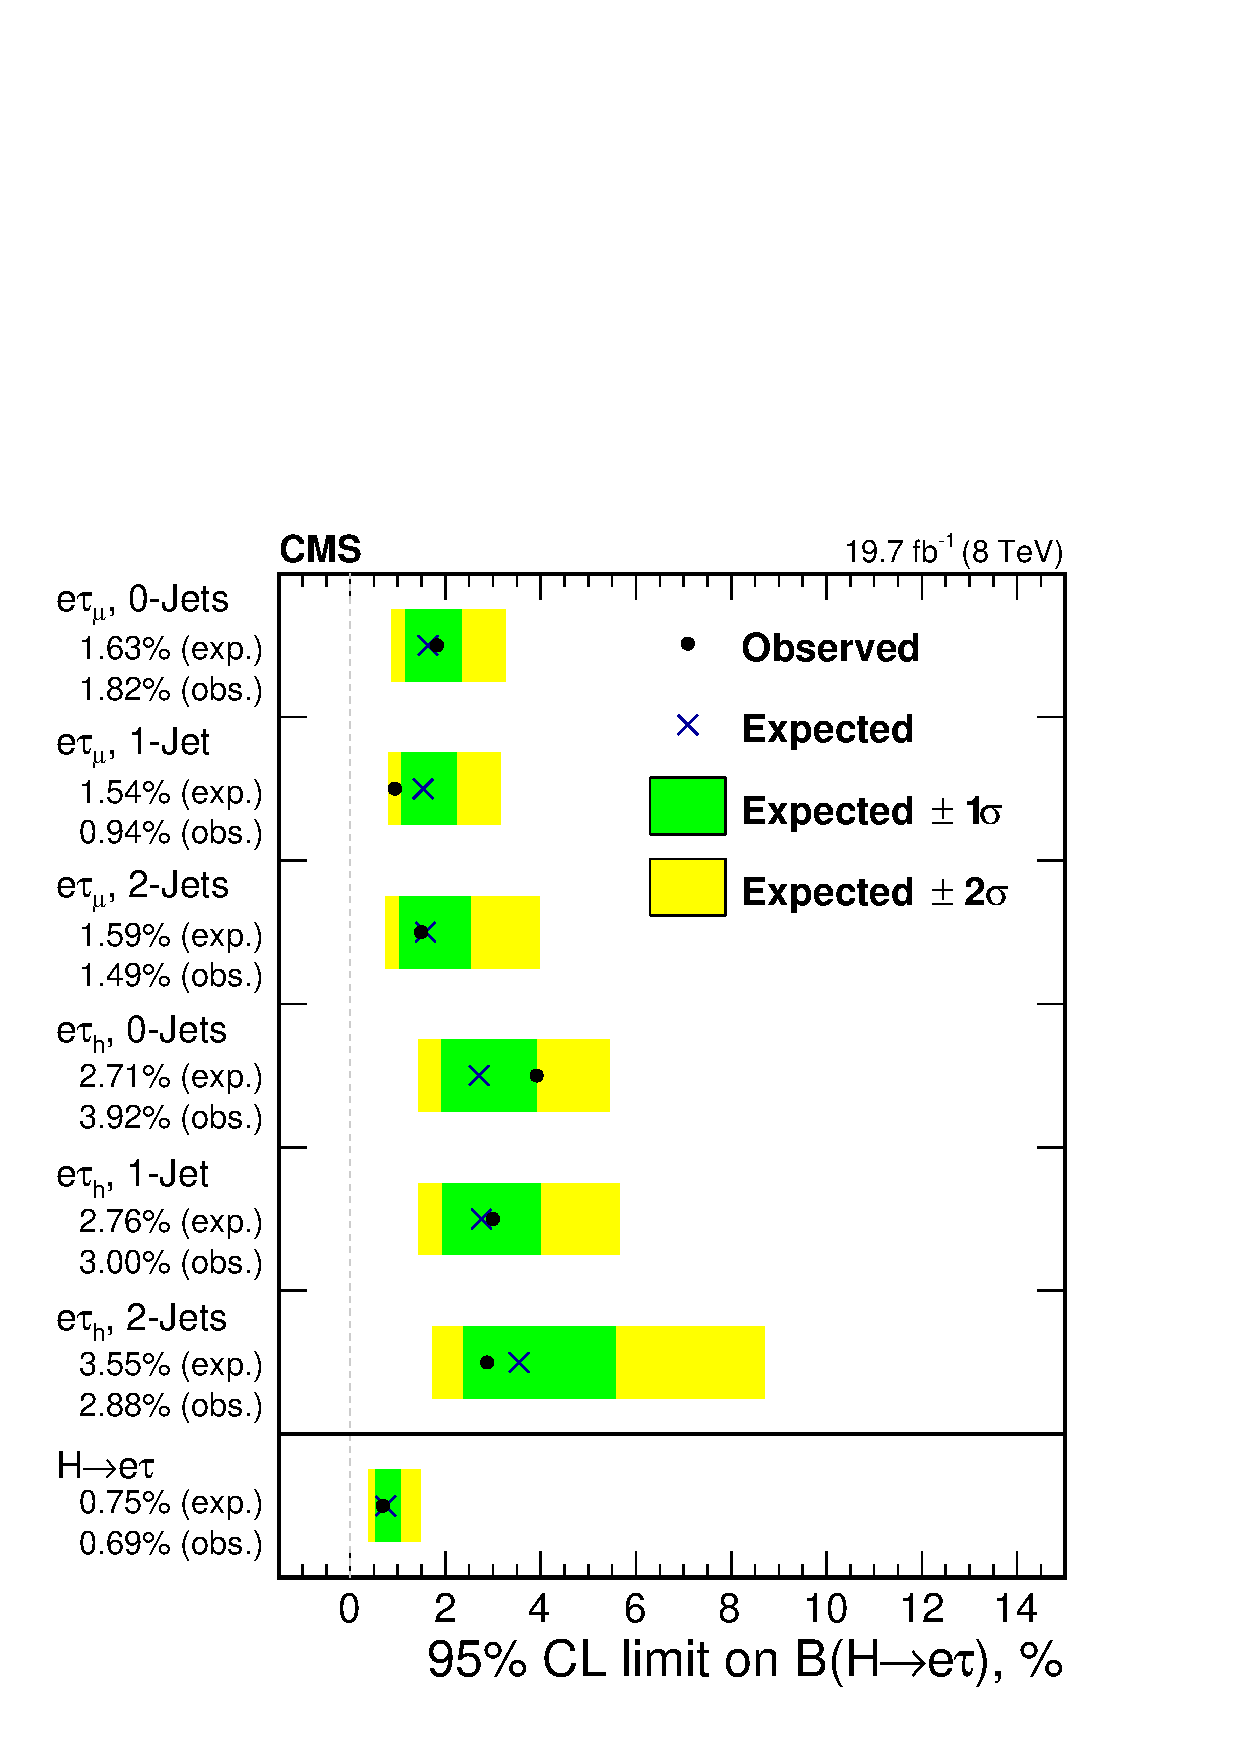
\includegraphics[width=0.6\textwidth]{chapter8/HEtau_summary.pdf}
\end{center}
\caption{95\% CL upper limit on branching ratio on $H \to e \tau$ with both the results from $\Hehad$ and $H \to e \tau_{\mu}$ and the combined. }

\label{fig:Etaulimitsummary}
\end{figure}


\begin{figure}[htpb]
\begin{center}
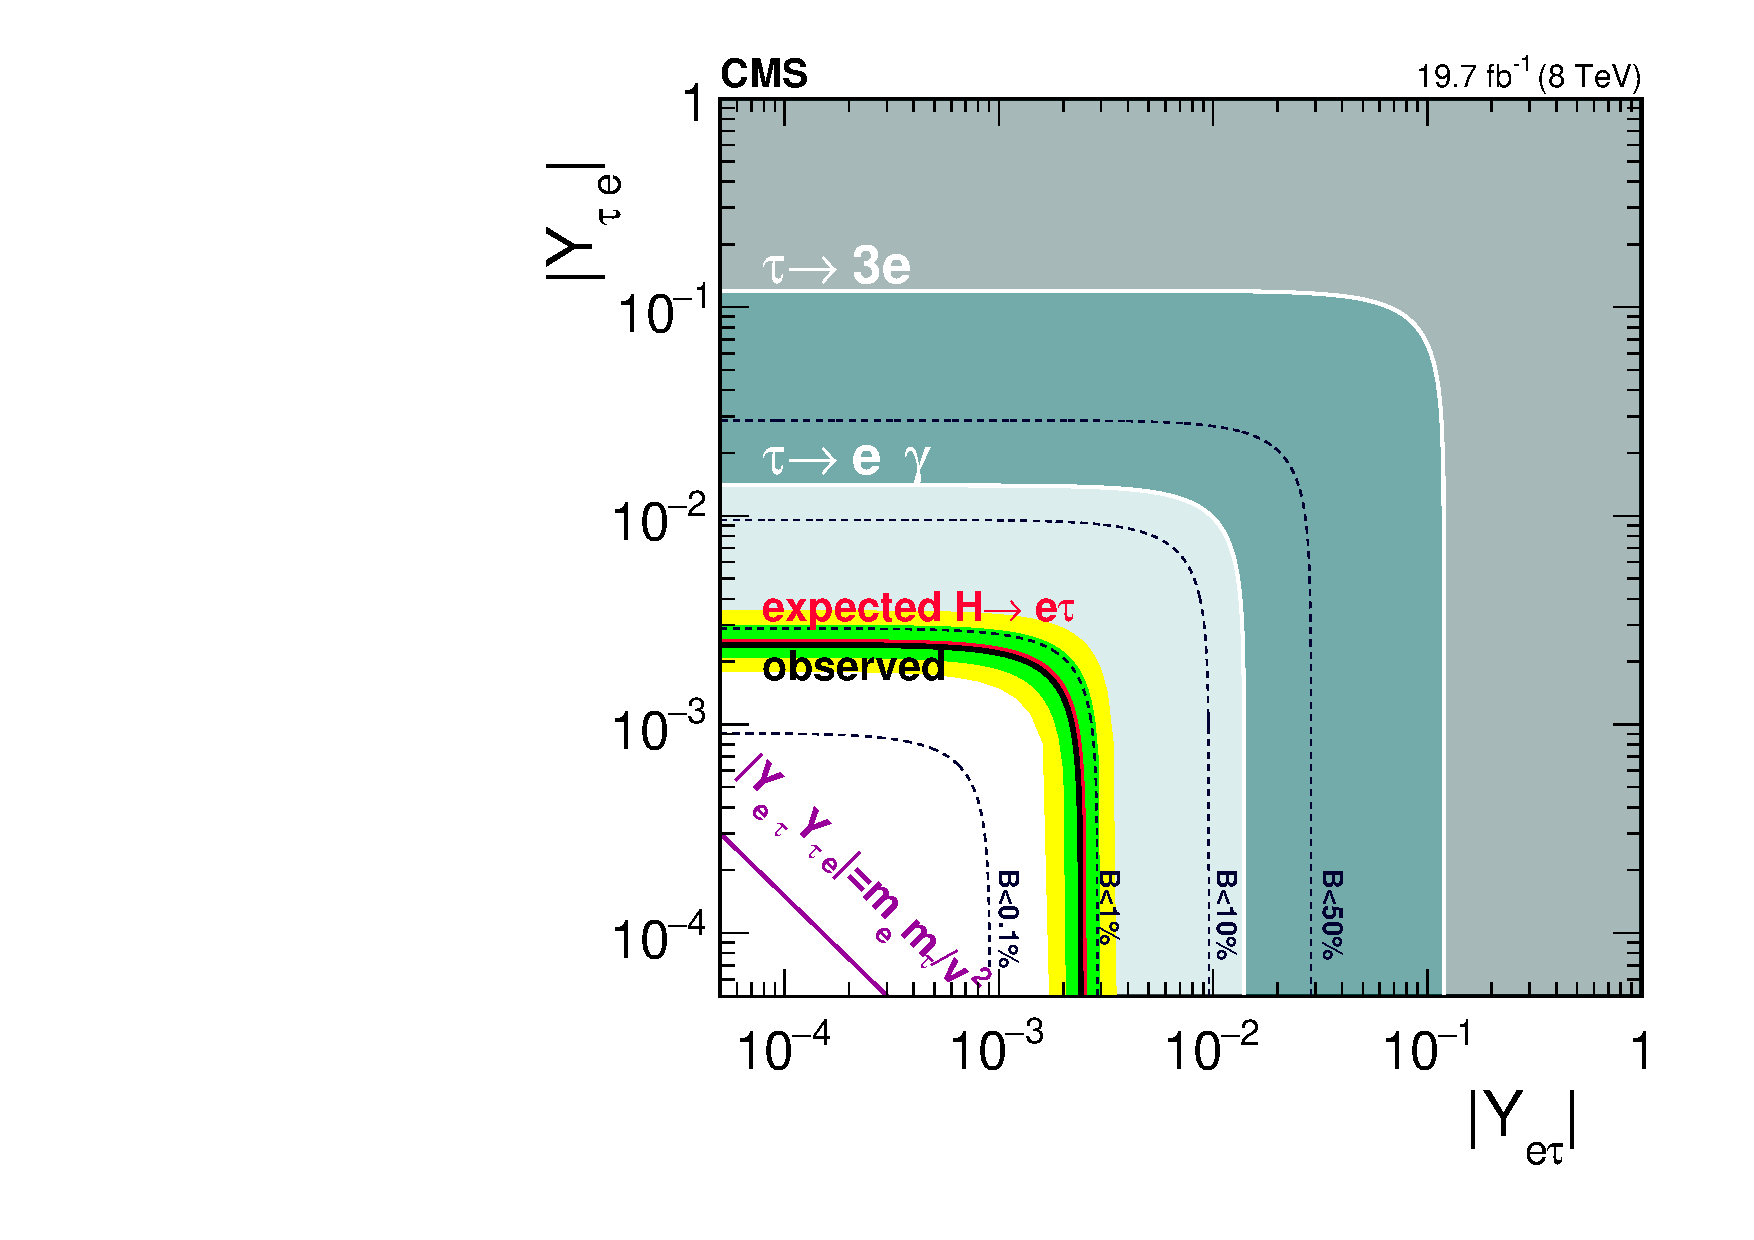
\includegraphics[width=0.6\textwidth]{chapter8/EtauYukawa.pdf}\label{fig:etauYukawa}
\end{center}

\caption[Upper limit of flavour violating Yukawa coupling in $H\to e\tau$ analysis]{Upper limit of flavour violating Yukawa coupling $|Y_{e\tau}|, |Y_{\tau e}|$ from the combined $H \to e \tau$ result. The red solid line represents the expected limit and the black solid line is the observed limit. 68\% and 95\% range of containing the observed limit is shown in the green and yellow band. The result from $\tau \to 3e$ is shown in gray, the one from $\tau \to e\gamma$ is shown in dark green and presented analysis is in light blue. The theoretical naturalness limit $Y_{ij}Y_{ji} \leq m_im_j/v^2$ is shown by purple diagonal line~\cite{Harnik:2012pb}}.
\label{fig:etauYukawas}
\end{figure}




